% Options for packages loaded elsewhere
\PassOptionsToPackage{unicode}{hyperref}
\PassOptionsToPackage{hyphens}{url}
%
\documentclass[
]{book}
\usepackage{lmodern}
\usepackage{amssymb,amsmath}
\usepackage{ifxetex,ifluatex}
\ifnum 0\ifxetex 1\fi\ifluatex 1\fi=0 % if pdftex
  \usepackage[T1]{fontenc}
  \usepackage[utf8]{inputenc}
  \usepackage{textcomp} % provide euro and other symbols
\else % if luatex or xetex
  \usepackage{unicode-math}
  \defaultfontfeatures{Scale=MatchLowercase}
  \defaultfontfeatures[\rmfamily]{Ligatures=TeX,Scale=1}
\fi
% Use upquote if available, for straight quotes in verbatim environments
\IfFileExists{upquote.sty}{\usepackage{upquote}}{}
\IfFileExists{microtype.sty}{% use microtype if available
  \usepackage[]{microtype}
  \UseMicrotypeSet[protrusion]{basicmath} % disable protrusion for tt fonts
}{}
\makeatletter
\@ifundefined{KOMAClassName}{% if non-KOMA class
  \IfFileExists{parskip.sty}{%
    \usepackage{parskip}
  }{% else
    \setlength{\parindent}{0pt}
    \setlength{\parskip}{6pt plus 2pt minus 1pt}}
}{% if KOMA class
  \KOMAoptions{parskip=half}}
\makeatother
\usepackage{xcolor}
\IfFileExists{xurl.sty}{\usepackage{xurl}}{} % add URL line breaks if available
\IfFileExists{bookmark.sty}{\usepackage{bookmark}}{\usepackage{hyperref}}
\hypersetup{
  pdftitle={Curso do R do GIEU},
  pdfauthor={Alan R. Panosso},
  hidelinks,
  pdfcreator={LaTeX via pandoc}}
\urlstyle{same} % disable monospaced font for URLs
\usepackage{color}
\usepackage{fancyvrb}
\newcommand{\VerbBar}{|}
\newcommand{\VERB}{\Verb[commandchars=\\\{\}]}
\DefineVerbatimEnvironment{Highlighting}{Verbatim}{commandchars=\\\{\}}
% Add ',fontsize=\small' for more characters per line
\usepackage{framed}
\definecolor{shadecolor}{RGB}{248,248,248}
\newenvironment{Shaded}{\begin{snugshade}}{\end{snugshade}}
\newcommand{\AlertTok}[1]{\textcolor[rgb]{0.94,0.16,0.16}{#1}}
\newcommand{\AnnotationTok}[1]{\textcolor[rgb]{0.56,0.35,0.01}{\textbf{\textit{#1}}}}
\newcommand{\AttributeTok}[1]{\textcolor[rgb]{0.77,0.63,0.00}{#1}}
\newcommand{\BaseNTok}[1]{\textcolor[rgb]{0.00,0.00,0.81}{#1}}
\newcommand{\BuiltInTok}[1]{#1}
\newcommand{\CharTok}[1]{\textcolor[rgb]{0.31,0.60,0.02}{#1}}
\newcommand{\CommentTok}[1]{\textcolor[rgb]{0.56,0.35,0.01}{\textit{#1}}}
\newcommand{\CommentVarTok}[1]{\textcolor[rgb]{0.56,0.35,0.01}{\textbf{\textit{#1}}}}
\newcommand{\ConstantTok}[1]{\textcolor[rgb]{0.00,0.00,0.00}{#1}}
\newcommand{\ControlFlowTok}[1]{\textcolor[rgb]{0.13,0.29,0.53}{\textbf{#1}}}
\newcommand{\DataTypeTok}[1]{\textcolor[rgb]{0.13,0.29,0.53}{#1}}
\newcommand{\DecValTok}[1]{\textcolor[rgb]{0.00,0.00,0.81}{#1}}
\newcommand{\DocumentationTok}[1]{\textcolor[rgb]{0.56,0.35,0.01}{\textbf{\textit{#1}}}}
\newcommand{\ErrorTok}[1]{\textcolor[rgb]{0.64,0.00,0.00}{\textbf{#1}}}
\newcommand{\ExtensionTok}[1]{#1}
\newcommand{\FloatTok}[1]{\textcolor[rgb]{0.00,0.00,0.81}{#1}}
\newcommand{\FunctionTok}[1]{\textcolor[rgb]{0.00,0.00,0.00}{#1}}
\newcommand{\ImportTok}[1]{#1}
\newcommand{\InformationTok}[1]{\textcolor[rgb]{0.56,0.35,0.01}{\textbf{\textit{#1}}}}
\newcommand{\KeywordTok}[1]{\textcolor[rgb]{0.13,0.29,0.53}{\textbf{#1}}}
\newcommand{\NormalTok}[1]{#1}
\newcommand{\OperatorTok}[1]{\textcolor[rgb]{0.81,0.36,0.00}{\textbf{#1}}}
\newcommand{\OtherTok}[1]{\textcolor[rgb]{0.56,0.35,0.01}{#1}}
\newcommand{\PreprocessorTok}[1]{\textcolor[rgb]{0.56,0.35,0.01}{\textit{#1}}}
\newcommand{\RegionMarkerTok}[1]{#1}
\newcommand{\SpecialCharTok}[1]{\textcolor[rgb]{0.00,0.00,0.00}{#1}}
\newcommand{\SpecialStringTok}[1]{\textcolor[rgb]{0.31,0.60,0.02}{#1}}
\newcommand{\StringTok}[1]{\textcolor[rgb]{0.31,0.60,0.02}{#1}}
\newcommand{\VariableTok}[1]{\textcolor[rgb]{0.00,0.00,0.00}{#1}}
\newcommand{\VerbatimStringTok}[1]{\textcolor[rgb]{0.31,0.60,0.02}{#1}}
\newcommand{\WarningTok}[1]{\textcolor[rgb]{0.56,0.35,0.01}{\textbf{\textit{#1}}}}
\usepackage{longtable,booktabs}
% Correct order of tables after \paragraph or \subparagraph
\usepackage{etoolbox}
\makeatletter
\patchcmd\longtable{\par}{\if@noskipsec\mbox{}\fi\par}{}{}
\makeatother
% Allow footnotes in longtable head/foot
\IfFileExists{footnotehyper.sty}{\usepackage{footnotehyper}}{\usepackage{footnote}}
\makesavenoteenv{longtable}
\usepackage{graphicx,grffile}
\makeatletter
\def\maxwidth{\ifdim\Gin@nat@width>\linewidth\linewidth\else\Gin@nat@width\fi}
\def\maxheight{\ifdim\Gin@nat@height>\textheight\textheight\else\Gin@nat@height\fi}
\makeatother
% Scale images if necessary, so that they will not overflow the page
% margins by default, and it is still possible to overwrite the defaults
% using explicit options in \includegraphics[width, height, ...]{}
\setkeys{Gin}{width=\maxwidth,height=\maxheight,keepaspectratio}
% Set default figure placement to htbp
\makeatletter
\def\fps@figure{htbp}
\makeatother
\setlength{\emergencystretch}{3em} % prevent overfull lines
\providecommand{\tightlist}{%
  \setlength{\itemsep}{0pt}\setlength{\parskip}{0pt}}
\setcounter{secnumdepth}{5}
\usepackage{booktabs}
\usepackage{booktabs}
\usepackage{longtable}
\usepackage{array}
\usepackage{multirow}
\usepackage{wrapfig}
\usepackage{float}
\usepackage{colortbl}
\usepackage{pdflscape}
\usepackage{tabu}
\usepackage{threeparttable}
\usepackage{threeparttablex}
\usepackage[normalem]{ulem}
\usepackage{makecell}
\usepackage[]{natbib}
\bibliographystyle{apalike}

\title{Curso do R do GIEU}
\author{Alan R. Panosso}
\date{2020-10-14}

\begin{document}
\maketitle

{
\setcounter{tocdepth}{1}
\tableofcontents
}
\hypertarget{introduuxe7uxe3o}{%
\chapter{INTRODUÇÃO}\label{introduuxe7uxe3o}}

A Estatística Experimental tem como objetivo o estudo dos experimentos, isto é, seu planejamneto, execução, análise dos dados e interpretação dos resultados obtidos.

Vejamos então, alguns conceitos básicos necessários para um bom entendimento da estatística Experimental.

\textbf{Alguns conceitos básicos}

\textbf{POPULAÇÃO}

Boa parte do conhecimento humano está baseado em um número relativamente reduzido de informações. Isto é verdadeiro, tanto no que se refere aos problemas do cotidiano, como no que se refere à pesquisa científica.

Por definição \textbf{POPULAÇÃO} é o conjunto de elementos que têm em comum uma determinada característica. Todo o subconjunto não vazio e com menor número de elemento do que o conjunto definido como \textbf{população} constitui, por definição, uma \textbf{AMOSTRA} desta população.

Uma população em ecologia é o número total de indivíduos de uma determinada espécie em uma área definida. Por exemplo, o número total de lagartas de \emph{Spodoptera frugiperda} em uma cultura de milho constitui uma população. Esta população, embora finita, é considerada para fins de amostragem como uma população infinita.

Uma vez definida a unidade amostral (1 planta, um conjunto de 5 plantas, ou um quadrado no qual será contado o número de lagartas), a população pode ser considerada como um conjunto de unidades amostrais e um subconjunto tomado aleatoriamente deste subconjunto é chamado de \textbf{AMOSTRA ALEATÓRIA DE TAMANHO N}.

Assim sendo, as observações são obtidas através de contagens do número de indivíduos em cada unidade amostral. Estas observações são chamadas de \textbf{VARIÁVEL EM ESTUDO}.

\textbf{TRATAMENTO}

É o método, elemento ou material, cujo efeito se deseja medir ou comparar em um experimento. Por exemplo, um tratamento pode ser: Uma variedade de cana-de-açúcar, um híbrido de sorgo, uma dose de um adubo para a cultura do milho, um espaçamento para cultura do algodão, um recipiente para produção de mudas de eucalipto, um inseticida para controle de pragas, etc.

\textbf{EXPERIMENTO OU ENSAIO}

Experimento é um trabalho previamente planejado, no qual se faz comparação dos efeitos dos tratamentos.

\textbf{UNIDADE EXPERIMENTAL OU PARCELA}

É a unidade na qual o tratamento é aplicado. É na parcela que obtemos os dados que deverão refletir o efeito de cada tratamento no ensaio. A parcela pode ser constituída por uma planta, uma área om um grupo de plantas, uma placa de petri com um meio de cultura, um animal, um lote de animais, etc.

\textbf{DELINEAMENTO EXPERIMENTAL}

É o plano utilizado na experimentação, e implica na forma como os tratamento deverão ser distribuídos nas unidades experimentais e como serão analisados os dados a serem obtidos. Como exemplo, temos o delineamento inteiramente casualizado (DIC), o delineamento em blocos casualizados (DBC) o delineamento em quadrado latino (DQL), entre outros.

\hypertarget{delineamento-inteiramente-casualizado}{%
\chapter{Delineamento Inteiramente Casualizado}\label{delineamento-inteiramente-casualizado}}

\textbf{Caracterização}

O delineamento inteiramente casualizado é o mais simples de todos os delineamentos experimentais, e os experimentos instalados de acordo com este delineamento são chamado de experimentos interiamente casualizados ou experimentos inteiramente ao acaso.

Este delineamento apresenta as seguintes características:

\begin{enumerate}
\def\labelenumi{\arabic{enumi}.}
\item
  Leva em consideração os princípios da \textbf{repetição} e da \textbf{casualização}, deixando de lado o princípio do controle local e, portanto, as repetições não são organizadas em blocos.
\item
  Os tratamentos são designados às parcelas de forma inteiramente casual, com qualquer número de repetições.
\end{enumerate}

\textbf{As principais vantagens desse delineamento são as seguintes:}

\begin{enumerate}
\def\labelenumi{\arabic{enumi})}
\item
  Flexibilidade, uma vez que o número de repetições pode variar de um tratamento para outro, sem causar sérios problemas na análise.
\item
  Proporciona o maior número de graus de liberdade possível para o resíduo.
\end{enumerate}

\textbf{As principais desvantagens desse delineamento são:}

\begin{enumerate}
\def\labelenumi{\arabic{enumi})}
\item
  As parcelas experimentais devem ser homogêneas.
\item
  Leva a uma alta estimativa da variância residual \(QM_{Res}\), uma vez que todas as variações, exceto aquela devido ao efeito de tratamentos, são tomadas como variação do acaso.
\end{enumerate}

Para a instalação desse experimento devemos ter certeza da homogeneidade das condições experimentais. Este delineamento é bastante utilizado em ensaios de laboratório e em ensaios com vasos, realizados dentro de casas de vegetação, em que as condições experimentais podem ser perfeitamente controladas.

A distribuição casual dos tratamentos a todas as parcelas do experimento é a principal característica deste delineamento. Por exemplo, num experimento no delineamento inteiramente casualizado com 5 tratamentos e 5 repetições, a casualização dos tratamentos seria feita sorteando-se para cada uma das 20 parcelas do experimento uma combinação de tratamento e repetição, ou seja:

\[
\begin{matrix}
A1 & A2 & A3 & A4 \\
B1 & B2 & B3 & B4 \\
C1 & C2 & C3 & C4 \\
D1 & D2 & D3 & D4 \\
E1 & E2 & E3 & E4 
\end{matrix}
\]

Assim, um sorteio para distribuição dos tratamento às parcelas poderia ser o seguinte:

\[
\begin{matrix}
B4 & D1 & B1 & A2 & D4\\
D2 & A1 & C4 & D3 & B3\\
E1 & E3 & B2 & C2 & C2\\
A4 & C1 & E4 & E2 & E2
\end{matrix}
\]

\textbf{Modelo Matemático}

Todo delineamento experimental possui um modelo matemático que o representa, que deve ser levado em conta na análise de variância, \textbf{aceitando algumas hipóteses básicas necessárias para a validade da análise.} No caso do DIC.

\[
x_{ij}= \mu + \tau_i + \epsilon_{ij}
\]
onde:
\(x{ij}\): é o valor observado na parcela que recebeu o tratamento \emph{i} na repetição \emph{j},

\(\mu\): é a média geral do experimento,

\(\tau_i\) é o efeito devido ao tratamento \emph{i} que foi aplicado à parcela,

\(\epsilon_{ij}\) é o efeito dos fatores não controlados na parcela que recebeu o tratamento \emph{i} na repetição \emph{j}.

\textbf{Hipóteses básicas para aplicação da análoise de variância}

As hipóteses básicas que devemos admitir para tornar válida a aplicação da análise de variância são as seguintes:

\begin{enumerate}
\def\labelenumi{\arabic{enumi})}
\item
  \textbf{Aditividade}: Os efeitos dos fatores do modelo são aditivos.
\item
  \textbf{Independência}: Os erros (desvios) \(\epsilon_{ij}\), devido aos efeitos de fatores não controlados ou acaso devem ser independentes.
\item
  \textbf{Homocedasticidade (homogeneidade de variâncias)}: Os erros (desvios) \(\epsilon_{ij}\), devido ao acaso devem possuir variância comum \(\sigma^2\)
\item
  \textbf{Normalidade dos desvios}: Os erros ou desvios \(\epsilon_{ij}\) devido ao acaso devem possuir distribuição normal de probabilidades.
\end{enumerate}

Uma forma resumida de apresentar estas quatro pressuposições é apresentada a seguir:

\[
\epsilon_{ij} \overset{iid}{\tilde{}} N(0,\sigma^2) \\
\]

\textbf{Exemplo de aplicação DIC}

Num experimento inteiramente casualizado, de competição de variedades de mandioca, realizado numa área perfeitamente homogênea quanto às condições experimentais, foram utilizadas 5 repetições das seguintes variedades:

1 - IAC 5

2 - IAC 7

3 - IAC 11

4 - IRACEMA

5 - MANTIQUEIRA

A designação dos tratamentos às parcelas no campo, juntamente com as produções, expressa em t/ha, foi a seguinte:

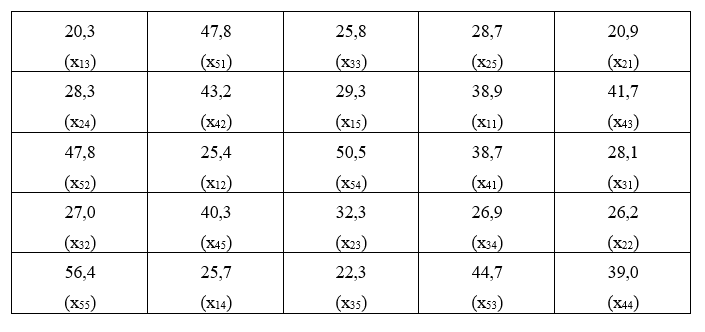
\includegraphics{Delin1.png}

Com estes dados, podemos organizar o quadro seguinte:

\begin{longtable}[]{@{}lcccccc@{}}
\toprule
Tratamentos & Rep.1 & Rep.2 & Rep.3 & Rep.4 & Rep.~5 & Total\tabularnewline
\midrule
\endhead
1 - IAC 5 & 38,9 & 25,4 & 20,3 & 25,7 & 29,3 & 139,6\tabularnewline
2 - IAC 7 & 20,9 & 26,2 & 32,3 & 28,3 & 28,7 & 136,4\tabularnewline
3 - IAC 11 & 28,1 & 27,0 & 25,8 & 26,9 & 22,3 & 130,1\tabularnewline
4 - IRACEMA & 38,7 & 43,2 & 41,7 & 39,0 & 40,3 & 202,9\tabularnewline
5 - MANTIQUEIRA & 47,8 & 47,8 & 44,7 & 50,5 & 56,4 & 247,2\tabularnewline
\textbf{Total} & & & & & & \textbf{856,2}\tabularnewline
\bottomrule
\end{longtable}

As hipóteses que desejamos testar são:

\(H_0\): As variedades de mandioca testadas não são diferentes entre si quanto à produção.

\(H_1\): As variedades de mandioca testadas diferem entre si quanto à produção.

\textbf{Aplicação no R - DIC}

Utilizando o R para obtermos o quadro da análise de variância, os dados estão disponíveis online em: \href{https://raw.githubusercontent.com/arpanosso/curso_GIEU/master/dados/mandioca.txt}{Mandioca}.


\includegraphics{Rlogo.png}

\begin{Shaded}
\begin{Highlighting}[]
\CommentTok{# Carregando o pacote para a análise}
\KeywordTok{library}\NormalTok{(ExpDes.pt)}
\KeywordTok{library}\NormalTok{(tidyverse)}


\CommentTok{# Caminho dos dados}
\NormalTok{caminho<-}\StringTok{"https://raw.githubusercontent.com/arpanosso/curso_GIEU/master/dados/mandioca.txt"}

\CommentTok{# Lendo o arquivo de dados}
\NormalTok{dados<-}\KeywordTok{read.table}\NormalTok{(caminho,}\DataTypeTok{h=}\NormalTok{T,}\DataTypeTok{sep=}\StringTok{"}\CharTok{\textbackslash{}t}\StringTok{"}\NormalTok{)}

\CommentTok{# verificando os 6 primeiros registros}
\KeywordTok{head}\NormalTok{(dados)}
\end{Highlighting}
\end{Shaded}

\begin{verbatim}
##   Trat Rep    Y
## 1    1   1 38.9
## 2    1   2 25.4
## 3    1   3 20.3
## 4    1   4 25.7
## 5    1   5 29.3
## 6    2   1 20.9
\end{verbatim}

\begin{Shaded}
\begin{Highlighting}[]
\CommentTok{# Análise de variância e teste de Tukey com a função dic}
\NormalTok{trat <-}\StringTok{ }\NormalTok{dados}\OperatorTok{$}\NormalTok{Trat }\CommentTok{# Criando o vetor de tratamentos}
\NormalTok{prod <-}\StringTok{ }\NormalTok{dados}\OperatorTok{$}\NormalTok{Y }\CommentTok{# Criando o vetor com a variável resposta}

\CommentTok{# Utilizando a função}
\KeywordTok{dic}\NormalTok{(trat,prod,}\DataTypeTok{mcomp =} \StringTok{"tukey"}\NormalTok{)}
\end{Highlighting}
\end{Shaded}

\begin{verbatim}
## ------------------------------------------------------------------------
## Quadro da analise de variancia
## ------------------------------------------------------------------------
##            GL      SQ QM     Fc      Pr>Fc
## Tratamento  4 2135.94  3 28.592 5.0773e-08
## Residuo    20  373.52  2                  
## Total      24 2509.46  1                  
## ------------------------------------------------------------------------
## CV = 12.62 %
## 
## ------------------------------------------------------------------------
## Teste de normalidade dos residuos 
## Valor-p:  0.2156065 
## De acordo com o teste de Shapiro-Wilk a 5% de significancia, os residuos podem ser considerados normais.
## ------------------------------------------------------------------------
## 
## ------------------------------------------------------------------------
## Teste de homogeneidade de variancia 
## valor-p:  0.1115615 
## De acordo com o teste de bartlett a 5% de significancia, as variancias podem ser consideradas homogeneas.
## ------------------------------------------------------------------------
## 
## Teste de Tukey
## ------------------------------------------------------------------------
## Grupos Tratamentos Medias
## a     5   49.44 
##  b    4   40.58 
##   c   1   27.92 
##   c   2   27.28 
##   c   3   26.02 
## ------------------------------------------------------------------------
\end{verbatim}

\hypertarget{delineamento-em-blocos-casualizados}{%
\chapter{Delineamento em Blocos Casualizados}\label{delineamento-em-blocos-casualizados}}

\textbf{Caracterização}

O delineamento em blocos casualizados (DBC) é o mais utilizado dos delineamentos experimentais, e os experimentos instalados de acordo com esse delineamento são denominados de \textbf{experimentos em blocos casualizados} ou \textbf{experimentos em blocos ao acaso}. Além dos princípios da \textbf{\emph{repetição}} e da \textbf{\emph{casualização}}, leva em conta também o princípio do \textbf{\emph{controle local}}.

Sempre que houver dúvidas a respeito da homogeneidade das condições experimentais é conveniente usar o princípio do controle local, estabelecendo blocos com parcelas homogêneas.

\textbf{As principais características deste delineamento são}:

\begin{enumerate}
\def\labelenumi{\arabic{enumi}.}
\item
  As parcelas são distribuídas em grupos ou blocos (princípio do controle local) de tal forma que elas sejam o mais uniforme possível dentro de cada bloco.
\item
  O número de parcelas por bloco deve ser igual ao número de tratamentos (blocos completos casualizados).
\item
  Os tratamentos são designados às parcelas de forma casual, sendo essa casualização feita dentro de cada bloco.
\end{enumerate}

Esse delineamento é mais eficiente que o delineamento inteiramente casualizado, e essa eficiência depende da uniformidade das parcelas dentro de cada bloco, podendo inclusive, haver diferenças acentuadas de um bloco para outro.

Então, por exemplo, se temos um experimento em blocos casualizados em que desejamos estudar o efeito de 4 variedades (V1,V2,V3 e V4), sendo cada uma delas repetidas 5 vezes, teremos o seguinte plano experimental:

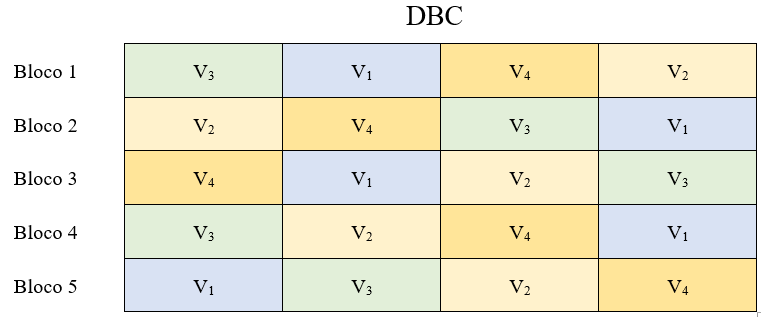
\includegraphics{DBC_d.png}

Note que dentro de cada bloco temos as variedades sorteadas ao acaso. Caso este mesmo ensaio fosse montado no delineamento inteiramente casualizados, o sorteio seria feito em todas as parcelas do experimento, e os tratamentos não seriam agrupados em blocos. Por exemplo, no delineamento inteiramente casualizado teríamos:

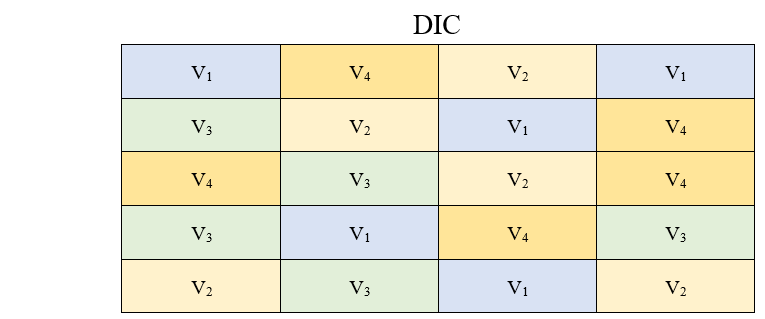
\includegraphics{DIC_d.png}

\textbf{As principais vantagens desse delineamento são:}

\begin{enumerate}
\def\labelenumi{\arabic{enumi}.}
\item
  Controla as diferenças que ocorrem nas condições experimentais de um bloco para outro.
\item
  Permite, dentro de certos limites, utilizar qualquer número de tratamentos e blocos.
\item
  Nos conduz a uma estimativa mais exata para a variância residual.
\item
  A análise de variância é relativamente simples, sendo apenas um pouco mais demorada que a do delineamento inteiramente casualizado, pois possui uma causa de variação a mais (Blocos).
\end{enumerate}

\textbf{As principais desvantagens desse delineamento são:}

\begin{enumerate}
\def\labelenumi{\arabic{enumi}.}
\item
  Pela utilização do princípio do controle local há uma diminuição no número de graus de liberdade do resíduo.
\item
  A exigência de homogeneidade dentro do bloco limita o número de tratamentos, que não pode ser muito grande.
\end{enumerate}

\textbf{Modelo matemático}

Para podermos analisar um experimento em qualquer delineamento, necessitamos conhecer o modelo matemático do mesmo, e aceitar algumas hipóteses básicas necessárias para a validade da análise de variância.

O modelo matemático do delineamento em blocos casualizados é o seguinte:

\[
x_{ij} = \mu +\tau_i + \beta_j+\epsilon_{ij}
\]

onde,
\(x_{ij}\) representa o valor esperado na parcela que recebeu o tratamento \(i\) e que se encontra no bloco \(j\).

\(\mu\) é a média geral do experimento.

\(\tau_i\) é o efeito devido ao tratamento \emph{i} que foi aplicado à parcela.

\(\beta_j\) é o efeito devido ao bloco \emph{j} em que se encontra a parcela.

\(\epsilon_{ij}\) é o efeito dos fatores não controlados ou acaso na parcela que recebeu o tratamento \emph{i} e que se encontra no bloco \emph{j}.

\textbf{CRITÉRIO DO TESTE}:

\textbf{Para Tratamentos}:

Comparamos o valor F calculado para tratamentos com o valor de F tabelado em função do número de GL de Tratamentos e GL do resíduo, ao nível \(\alpha\) de significância.

Se \(F_{Trat} > F_{Tab}\), concluímos que o teste é significativo, portanto, rejeitamos \(H_0\) e devemos concluir que existe diferença significativa entre os efeitos dos tratamentos testados em relação à variáveis (característica) em estudo.

\textbf{Para Blocos}:

Pra Blocos, a comparação é feita entre o valor de F calculado com o F tabelado em função do número de GL de Blocos e GL do resíduo, ao nível \(\alpha\) de significância

Se \(F_{Blocos} > F_{Tab}\), concluímos que o teste é significativo, portanto, rejeitamos \(H_0\) e devemos concluir que os blocos possuem efeitos diferentes em relação à característica em estudo, ou seja, os blocos foram eficientes no controle da heterogeneidade local.

\textbf{Exemplo de aplicação do DBC}

No trabalho ``Influência do genótipo e da adubação sobre algumas características fenotípicas de \emph{Zea mays} L (Milho)'', realizado por BARBOSA (1976), foram utilizadas 4 cultivares de milho:

\(C_1\) = OPACO 2

\(C_2\) = PIRANÃO

\(C_3\) = COMPOSTO FLINT

\(C_4\) = AGROCERES AG-152

O ensaio foi montado de acordo com o delineamento em blocos casualizados, sendo utilizados 5 blocos para controlar as diferenças de fertilidade do solo entre terraços.

Os resultados obtidos para a produção em kg/ha, foram os seguintes e podem ser encontrados online em \href{https://raw.githubusercontent.com/arpanosso/curso_GIEU/master/dados/milho.txt}{milho}.

\begin{table}[H]
\centering
\begin{tabular}{l|r|r|r|r|r|>{}r}
\hline
Tratamentos & Bloco1 & Bloco2 & Bloco3 & Bloco4 & Bloco5 & Total\\
\hline
OPACO2 & 2812 & 2296 & 3501 & 3301 & 3691 & \cellcolor{lightgray}{\textcolor{black}{\textbf{15601}}}\\
\hline
PIRANAO & 3728 & 3588 & 4418 & 4544 & 5084 & \cellcolor{lightgray}{\textcolor{black}{\textbf{21362}}}\\
\hline
COMP.FLINT & 5359 & 5106 & 7477 & 8007 & 7956 & \cellcolor{lightgray}{\textcolor{black}{\textbf{33905}}}\\
\hline
AG152 & 4482 & 4510 & 5236 & 5930 & 5025 & \cellcolor{lightgray}{\textcolor{black}{\textbf{25183}}}\\
\hline
\cellcolor{lightgray}{\textcolor{black}{\textbf{Total}}} & \cellcolor{lightgray}{\textcolor{black}{\textbf{16381}}} & \cellcolor{lightgray}{\textcolor{black}{\textbf{15500}}} & \cellcolor{lightgray}{\textcolor{black}{\textbf{20632}}} & \cellcolor{lightgray}{\textcolor{black}{\textbf{21782}}} & \cellcolor{lightgray}{\textcolor{black}{\textbf{21756}}} & \cellcolor{lightgray}{\textcolor{black}{\textbf{\textbf{96051}}}}\\
\hline
\end{tabular}
\end{table}

As hipóteses que desejamos testar são as seguintes:

\[
\begin{cases} H_0: As\;cultivares\;testadas\;não\;diferem\;entre\;si\;em\;relação\;à\;produção\;da\;cultura\;do\;milho. \\
H_1: As\;cultivares\;testadas\;diferem\;entre\;si\;em\;relação\;à\;produção\;da\;cultura\;do\;milho.
\end{cases}
\]

\textbf{Aplicação em R - DBC}


\includegraphics{R.png}

\begin{Shaded}
\begin{Highlighting}[]
\NormalTok{dados<-}\KeywordTok{read.table}\NormalTok{(caminho,}\DataTypeTok{h=}\NormalTok{T,}\DataTypeTok{sep=}\StringTok{"}\CharTok{\textbackslash{}t}\StringTok{"}\NormalTok{)}
\KeywordTok{head}\NormalTok{(dados)}
\end{Highlighting}
\end{Shaded}

\begin{verbatim}
##      trat bloco    y
## 1  OPACO2     1 2812
## 2  OPACO2     2 2296
## 3  OPACO2     3 3501
## 4  OPACO2     4 3301
## 5  OPACO2     5 3691
## 6 PIRANAO     1 3728
\end{verbatim}

\begin{Shaded}
\begin{Highlighting}[]
\CommentTok{# Extraindo os fatores e a variável resposta}
\NormalTok{trat<-}\KeywordTok{as.factor}\NormalTok{(dados}\OperatorTok{$}\NormalTok{trat)}
\NormalTok{bloco<-}\KeywordTok{as.factor}\NormalTok{(dados}\OperatorTok{$}\NormalTok{bloco)}
\NormalTok{y<-dados}\OperatorTok{$}\NormalTok{y}

\CommentTok{# Definindo o modelo matemático}
\NormalTok{modelo<-}\KeywordTok{aov}\NormalTok{(y}\OperatorTok{~}\NormalTok{trat}\OperatorTok{+}\NormalTok{bloco)}
\KeywordTok{anova}\NormalTok{(modelo)}
\end{Highlighting}
\end{Shaded}

\begin{verbatim}
## Analysis of Variance Table
## 
## Response: y
##           Df   Sum Sq  Mean Sq F value    Pr(>F)    
## trat       3 35402022 11800674 44.3450 9.068e-07 ***
## bloco      4  9221681  2305420  8.6634   0.00158 ** 
## Residuals 12  3193330   266111                      
## ---
## Signif. codes:  0 '***' 0.001 '**' 0.01 '*' 0.05 '.' 0.1 ' ' 1
\end{verbatim}

\begin{Shaded}
\begin{Highlighting}[]
\CommentTok{#Comparação de Médias pelo teste de Tukey}
\KeywordTok{require}\NormalTok{(}\StringTok{"agricolae"}\NormalTok{)}
\end{Highlighting}
\end{Shaded}

\begin{verbatim}
## Loading required package: agricolae
\end{verbatim}

\begin{verbatim}
## 
## Attaching package: 'agricolae'
\end{verbatim}

\begin{verbatim}
## The following objects are masked from 'package:ExpDes.pt':
## 
##     lastC, order.group, tapply.stat
\end{verbatim}

\begin{Shaded}
\begin{Highlighting}[]
\NormalTok{glRes<-}\KeywordTok{df.residual}\NormalTok{(modelo)}
\NormalTok{QMres<-}\KeywordTok{deviance}\NormalTok{(modelo)}\OperatorTok{/}\NormalTok{glRes}
\NormalTok{tukey <-}\StringTok{ }\KeywordTok{HSD.test}\NormalTok{(modelo,}\StringTok{"trat"}\NormalTok{, }\DataTypeTok{group=}\OtherTok{TRUE}\NormalTok{,}\DataTypeTok{console=}\OtherTok{TRUE}\NormalTok{)}
\end{Highlighting}
\end{Shaded}

\begin{verbatim}
## 
## Study: modelo ~ "trat"
## 
## HSD Test for y 
## 
## Mean Square Error:  266110.8 
## 
## trat,  means
## 
##                 y       std r  Min  Max
## AG152      5036.6  596.4368 5 4482 5930
## COMP.FLINT 6781.0 1431.4177 5 5106 8007
## OPACO2     3120.2  565.1997 5 2296 3691
## PIRANAO    4272.4  616.1240 5 3588 5084
## 
## Alpha: 0.05 ; DF Error: 12 
## Critical Value of Studentized Range: 4.19866 
## 
## Minimun Significant Difference: 968.628 
## 
## Treatments with the same letter are not significantly different.
## 
##                 y groups
## COMP.FLINT 6781.0      a
## AG152      5036.6      b
## PIRANAO    4272.4      b
## OPACO2     3120.2      c
\end{verbatim}

\begin{Shaded}
\begin{Highlighting}[]
\KeywordTok{bar.group}\NormalTok{(tukey}\OperatorTok{$}\NormalTok{groups,}
          \DataTypeTok{las=}\DecValTok{1}\NormalTok{,}
          \DataTypeTok{ylim=}\KeywordTok{c}\NormalTok{(}\DecValTok{0}\NormalTok{,}\KeywordTok{max}\NormalTok{(y)}\OperatorTok{*}\FloatTok{1.10}\NormalTok{),}
          \DataTypeTok{xlab=}\StringTok{"Cultivares"}\NormalTok{,}
          \DataTypeTok{ylab=}\StringTok{"Produção (kg por ha)"}\NormalTok{,}
          \DataTypeTok{main=}\StringTok{"Teste de Tukey (5%)"}\NormalTok{);}\KeywordTok{box}\NormalTok{()}
\end{Highlighting}
\end{Shaded}

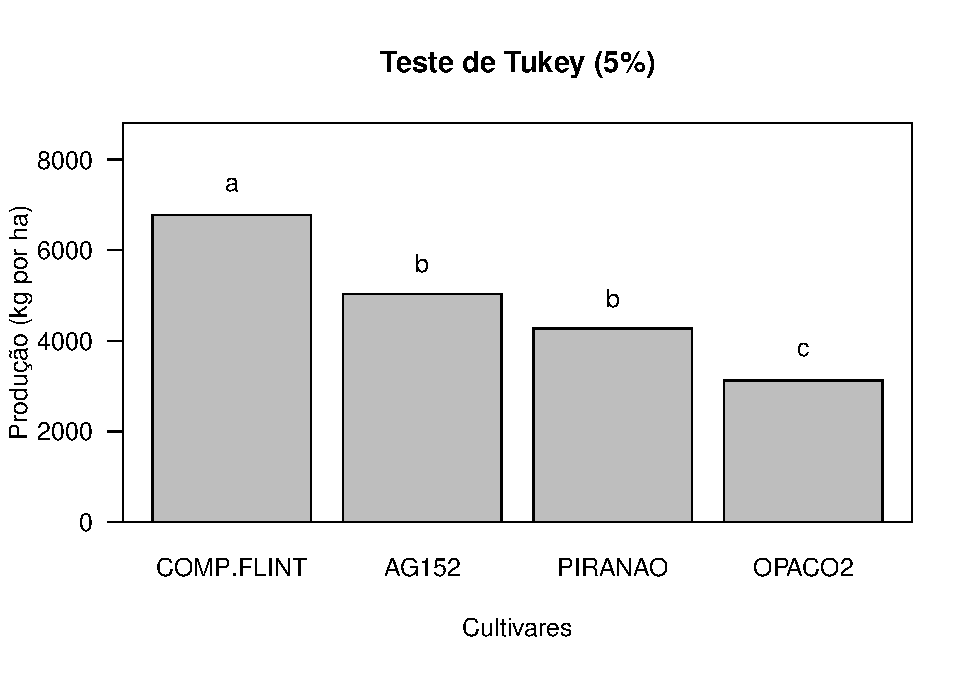
\includegraphics{curso_GIEU_files/figure-latex/unnamed-chunk-3-1.pdf}

\begin{Shaded}
\begin{Highlighting}[]
\CommentTok{# Cálculo do CV}
\NormalTok{cv<-}\DecValTok{100}\OperatorTok{*}\KeywordTok{sqrt}\NormalTok{(QMres)}\OperatorTok{/}\KeywordTok{mean}\NormalTok{(y)}
\KeywordTok{paste}\NormalTok{(}\KeywordTok{round}\NormalTok{(cv,}\DecValTok{2}\NormalTok{),}\StringTok{"%"}\NormalTok{,}\DataTypeTok{sep=}\StringTok{""}\NormalTok{)}
\end{Highlighting}
\end{Shaded}

\begin{verbatim}
## [1] "10.74%"
\end{verbatim}

Utilizando o pacote ``ExpDes.pt''

\begin{Shaded}
\begin{Highlighting}[]
\CommentTok{# Carregando o pacote para a análise}
\KeywordTok{library}\NormalTok{(ExpDes.pt)}

\CommentTok{# verificando os 6 primeiros registros}
\KeywordTok{head}\NormalTok{(dados)}
\end{Highlighting}
\end{Shaded}

\begin{verbatim}
##      trat bloco    y
## 1  OPACO2     1 2812
## 2  OPACO2     2 2296
## 3  OPACO2     3 3501
## 4  OPACO2     4 3301
## 5  OPACO2     5 3691
## 6 PIRANAO     1 3728
\end{verbatim}

\begin{Shaded}
\begin{Highlighting}[]
\CommentTok{# Análise de variância e teste de Tukey com a função dbc}
\NormalTok{trat <-}\StringTok{ }\NormalTok{dados}\OperatorTok{$}\NormalTok{trat }\CommentTok{# Criando o vetor de tratamentos}
\NormalTok{bloco <-}\StringTok{ }\NormalTok{dados}\OperatorTok{$}\NormalTok{bloco }\CommentTok{# Criando o vetor dos blocos}
\NormalTok{y <-}\StringTok{ }\NormalTok{dados}\OperatorTok{$}\NormalTok{y }\CommentTok{# Criando o vetor com a variável resposta}

\CommentTok{# Utilizando a função}
\KeywordTok{dbc}\NormalTok{(trat,bloco,y,}\DataTypeTok{mcomp =} \StringTok{"tukey"}\NormalTok{)}
\end{Highlighting}
\end{Shaded}

\begin{verbatim}
## ------------------------------------------------------------------------
## Quadro da analise de variancia
## ------------------------------------------------------------------------
##            GL       SQ QM     Fc      Pr>Fc
## Tratamento  3 35402022  2 44.345 0.00000091
## Bloco       4  9221681  3  8.663 0.00158020
## Residuo    12  3193330  4                  
## Total      19 47817033  1                  
## ------------------------------------------------------------------------
## CV = 10.74 %
## 
## ------------------------------------------------------------------------
## Teste de normalidade dos residuos 
## valor-p:  0.1786606 
## De acordo com o teste de Shapiro-Wilk a 5% de significancia, os residuos podem ser considerados normais.
## ------------------------------------------------------------------------
## 
## ------------------------------------------------------------------------
## Teste de homogeneidade de variancia 
## valor-p:  0.03461775 
## ATENCAO: a 5% de significancia, as variancias nao podem ser consideradas homogeneas!
## ------------------------------------------------------------------------
## 
## Teste de Tukey
## ------------------------------------------------------------------------
## Grupos Tratamentos Medias
## a     COMP.FLINT      6781 
##  b    AG152   5036.6 
##  b    PIRANAO     4272.4 
##   c   OPACO2      3120.2 
## ------------------------------------------------------------------------
\end{verbatim}

\hypertarget{experimentos-fatoriais}{%
\chapter{Experimentos Fatoriais}\label{experimentos-fatoriais}}

\textbf{Introdução}

Os experimentos simples, realizados de acordo com o delineamento interiamente casualizado ou em blocos casualizados, são utilizados para testar os efeitos de apenas um tipo de \textbf{tratamento}, ou \textbf{fator}, sendo os demais mantidos constantes.

Assim, por exemplo, num experimento de comparação de inseticidas em relação ao controle de uma determinada praga, devemos manter constante a dosagem, o método de aplicação, os tratos culturas, etc.

Porém, há casos em que necessitamos testar simultaneamente os efeitos de dois ou mais tipos de tratamentos (fatores) para obtermos resultados de interesse prático. Por exemplo, supondo que desejamos testar 3 inseticidas, 2 métodos de aplicação e 4 dosagens, teremos então um experimento fatorial de \(3\times2\times4\).

Os experimentos fatoriais são aqueles que nos permitem estudar, simultaneamente, os efeitos de dois ou mais tipos de fatores (tratamentos). Assim, eles devem ser instalados em um dos delineamentos já estudados (DIC, DBC, etc.).

Estes experimentos são utilizados em quase todos os campos de investigação e são bastante úteis em pesquisas iniciais, nas quais pouco se conhece a respeito de uma série de fatores.

\textbf{O número de tratamentos nos experimentos fatoriais consiste de todas as combinações possíveis dos níveis dos fatores}.

Por exemplo, se estamos interessados em testar o efeito de 3 inseticidas, cada um dos quais em 4 doses, teremos os 12 tratamentos seguintes.

\[
\begin{array}{} 
I_1 D_1  & I_2D_1  & I_3D_1 \\
I_1D_2  & I_2D_2  & I_3D_2 \\
I_1D_3  & I_2D_3  & I_3D_3 \\ 
I_1D_4  & I_2D_4  & I_3D_4 \end{array}
\]

Neste caso, representamos o esquema fatorial como: \(\text{Fatorial }3 \times 4\) com 3 inseticidas e 4 dosagens.

\textbf{As subdivisões de um fator são denominados NÍVEIS desse fator}. Então, no exemplo anterior, o fator \textbf{Inseticida} ocorrem em \textbf{3 níveis}, e o fator \textbf{Dosagem} ocorre em \textbf{4 nívies}. Assim, no ensaio acima, podemos obter conclusões sobre a qual o melhor inseticida, qual a melhor dosagem e qual a melhor dosagem para cada inseticida.

\textbf{Classificação dos Experementos Fatoriais}

\textbf{Fatoriais de série \(2^N\)}

Nesta série são enquadrados os experimentos fatoriais em que são estudados os efeitos de N fatores cada um em 2 níveis.

BASE = Nº de Níveis\\
EXPOENTE = Nº de Fatores

Exemplos:
\[
2^2 \Rightarrow \text{2 Fatores em 2 Níveis} \\
2^3 \Rightarrow \text{3 Fatores em 2 Níveis} \\
2^4 \Rightarrow \text{4 Fatores em 2 Níveis} \\
\]

etc.

\textbf{Fatoriais de série}

Nesta série são enquadrados os experimentos fatoriais em que são estudados os efeitos de N fatores cada um em 3 níveis.

Exemplos:
\[
3^2 \Rightarrow \text{2 Fatores em 3 Níveis} \\
3^3 \Rightarrow \text{3 Fatores em 3 Níveis} \\
3^4 \Rightarrow \text{4 Fatores em 3 Níveis} \\
\]
etc.

\textbf{Fatoriais de série mista}

Nesta série são enquadrado os fatoriais em que os fatores ocorrem em número diferente de níveis:

Exemplo:
\[
4\times 3\times 2 \Rightarrow \begin{cases} \text{1º Fator em 4 Níveis }\\ \text{2º Fator em 3 Níveis } \\ \text{3º Fator em 2 Níveis } \end{cases}
\]

\textbf{Casualização dos tratamentos}

Para exemplificar a casualização dos tratamentos, vamos supor um experimento fatorial \(3 \times 2\), com 3 variedades de milho (\(V_1,V_2,V_3\)) e 2 níveis de adubação dom \(P_2O_5\) (\(P_1 e\; P_2\)). Se o experimento fosee instalado de acordo com o delineamento em blocos casualizados, com 4 repetições, teríamos:

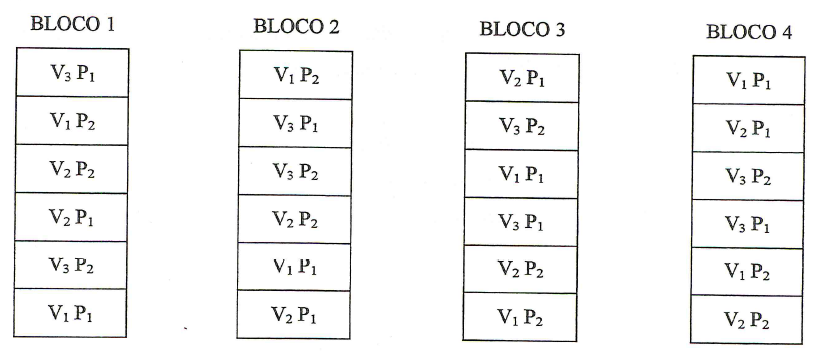
\includegraphics{Casuali.png}
\textbf{Análise de variância de um experimento fatorial com 2 fatores com interação não significativa}

Para a obtenção da análise de variância, vamos utlizar os dados adaptados do trabalho ``Ensaios em condições de casa-de-vegetação para controlo químico do `damping-off' em \emph{Eucalyptus saligna} Sm.'', realizado por KRUGNER; CARVALHO (1971) e publicado em IPEF, n 2/3 p.~97-113. O ensaio foi realizado no delineamento inteiramente casualizado, com 3 repetições e foram estudados os efeitos sobre a altura média das mudas de \emph{Eucalytus saligna}, do fatores:

\textbf{Tratamento do solo (S)}, sendo:\\
\(S_1=\text{Vapam}\)\\
\(S_2=\text{Brometo de metila}\)\\
\(S_3=\text{PCNB}\)\\
\(S_4=\text{Testemunha}\)

\textbf{Pulverização} com fungicida em pós emergência, sendo:\\
\(F_0 = \text{Sem fungicida}\)\\
\(F_1 = \text{Com fungicida}\)

As alturas médias de mudas (cm) 28 dias após a semeadura foram:

\begin{longtable}[]{@{}lcccr@{}}
\toprule
Tratamentos & Rep.1 & Rep.2 & Rep.3 & Total\tabularnewline
\midrule
\endhead
\(S_1F_0\) & 4,65 & 5,18 & 5,52 & 15,35\tabularnewline
\(S_1F_1\) & 4,86 & 4,81 & 4,51 & 14,18\tabularnewline
\(S_2F_0\) & 4,55 & 5,16 & 6,00 & 15,71\tabularnewline
\(S_2F_1\) & 4,73 & 5,51 & 5,09 & 15,33\tabularnewline
\(S_3F_0\) & 2,68 & 2,65 & 2,56 & 7,89\tabularnewline
\(S_3F_1\) & 2,90 & 2,71 & 2,93 & 8,54\tabularnewline
\(S_4F_0\) & 3,48 & 2,75 & 3,06 & 9,29\tabularnewline
\(S_4F_1\) & 2,65 & 2,47 & 2,83 & 7,95\tabularnewline
\textbf{Total} & & & & \textbf{94,24}\tabularnewline
\bottomrule
\end{longtable}

Os dados podem ser encontrados online em \href{https://raw.githubusercontent.com/arpanosso/curso_GIEU/master/dados/solofungi.txt}{solofungi.txt}

\textbf{Aplicação em R - Fatorial com Interação Não Significativa}


\includegraphics{R.png}

\textbf{Utilizando as funções básicas e o pacote agricolae}

\begin{Shaded}
\begin{Highlighting}[]
\CommentTok{# Carregando o pacote para análise de variância}
\KeywordTok{library}\NormalTok{(agricolae)}
\KeywordTok{library}\NormalTok{(tidyverse)}

\CommentTok{# Definindo o caminho do banco de dados}
\NormalTok{caminho<-}\StringTok{"https://raw.githubusercontent.com/arpanosso/curso_GIEU/master/dados/solofungi.txt"}

\CommentTok{# Entrada da dados}
\NormalTok{dados<-}\KeywordTok{read.table}\NormalTok{(caminho,}\DataTypeTok{h=}\OtherTok{TRUE}\NormalTok{)}

\CommentTok{#Guardando os fatores (tratamentos de solo e fungicidas) e a variável resposta (y)}
\NormalTok{solos<-}\KeywordTok{as.factor}\NormalTok{(dados}\OperatorTok{$}\NormalTok{S)}
\NormalTok{fungicida<-}\KeywordTok{as.factor}\NormalTok{(dados}\OperatorTok{$}\NormalTok{F)}
\NormalTok{y<-dados}\OperatorTok{$}\NormalTok{y}

\CommentTok{# Gráfico da interação}
\NormalTok{dados }\OperatorTok\StringTok{ }
\StringTok{  }\KeywordTok{group_by}\NormalTok{(S,F) }\OperatorTok\StringTok{ }
\StringTok{  }\KeywordTok{summarise}\NormalTok{(}\DataTypeTok{Y =} \KeywordTok{mean}\NormalTok{(y)) }\OperatorTok\StringTok{ }
\StringTok{  }\KeywordTok{ggplot}\NormalTok{(}\KeywordTok{aes}\NormalTok{(}\DataTypeTok{x=}\NormalTok{S, }\DataTypeTok{y=}\NormalTok{Y,}\DataTypeTok{col=}\KeywordTok{as.factor}\NormalTok{(F)))}\OperatorTok{+}
\StringTok{  }\KeywordTok{geom_line}\NormalTok{()}\OperatorTok{+}
\StringTok{  }\KeywordTok{labs}\NormalTok{(}\DataTypeTok{x=}\StringTok{"Tratamentos do solo"}\NormalTok{,}\DataTypeTok{y=}\StringTok{"Altura de plantas (cm)"}\NormalTok{,}\DataTypeTok{col=}\StringTok{"Fungicida"}\NormalTok{)}
\end{Highlighting}
\end{Shaded}

\begin{verbatim}
## `summarise()` regrouping output by 'S' (override with `.groups` argument)
\end{verbatim}

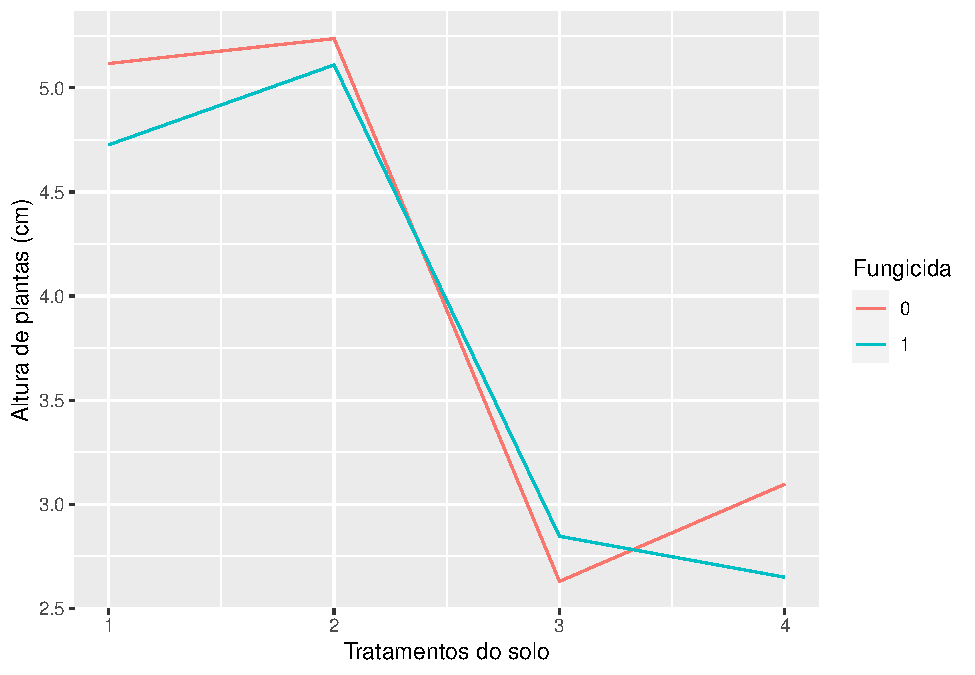
\includegraphics{curso_GIEU_files/figure-latex/unnamed-chunk-5-1.pdf}

\begin{Shaded}
\begin{Highlighting}[]
\NormalTok{dados }\OperatorTok\StringTok{ }
\StringTok{  }\KeywordTok{group_by}\NormalTok{(S,F) }\OperatorTok\StringTok{ }
\StringTok{  }\KeywordTok{summarise}\NormalTok{(}\DataTypeTok{Y =} \KeywordTok{mean}\NormalTok{(y)) }\OperatorTok\StringTok{ }
\StringTok{  }\KeywordTok{ggplot}\NormalTok{(}\KeywordTok{aes}\NormalTok{(}\DataTypeTok{x=}\NormalTok{F, }\DataTypeTok{y=}\NormalTok{Y,}\DataTypeTok{col=}\KeywordTok{as.factor}\NormalTok{(S)))}\OperatorTok{+}
\StringTok{  }\KeywordTok{geom_line}\NormalTok{()}\OperatorTok{+}
\StringTok{  }\KeywordTok{labs}\NormalTok{(}\DataTypeTok{x=}\StringTok{"Fungicida"}\NormalTok{,}\DataTypeTok{y=}\StringTok{"Altura de plantas (cm)"}\NormalTok{,}\DataTypeTok{col=}\StringTok{"Tratamentos do solo"}\NormalTok{)}
\end{Highlighting}
\end{Shaded}

\begin{verbatim}
## `summarise()` regrouping output by 'S' (override with `.groups` argument)
\end{verbatim}

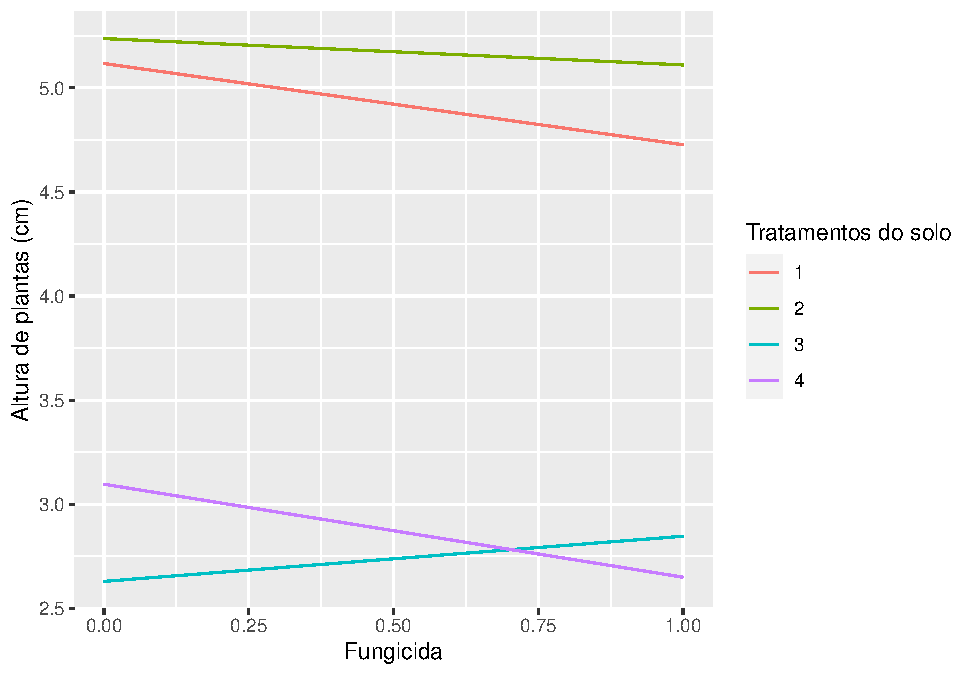
\includegraphics{curso_GIEU_files/figure-latex/unnamed-chunk-5-2.pdf}
\textbf{Analise considerando o delineamento de tratamentos}

\begin{Shaded}
\begin{Highlighting}[]
\NormalTok{mod <-}\StringTok{ }\KeywordTok{aov}\NormalTok{(y}\OperatorTok{~}\NormalTok{solos}\OperatorTok{+}\NormalTok{fungicida}\OperatorTok{+}\NormalTok{solos}\OperatorTok{:}\NormalTok{fungicida)}
\KeywordTok{anova}\NormalTok{(mod)}
\end{Highlighting}
\end{Shaded}

\begin{verbatim}
## Analysis of Variance Table
## 
## Response: y
##                 Df  Sum Sq Mean Sq F value   Pr(>F)    
## solos            3 30.3951 10.1317 74.0035 1.35e-09 ***
## fungicida        1  0.2091  0.2091  1.5271   0.2344    
## solos:fungicida  3  0.4128  0.1376  1.0051   0.4161    
## Residuals       16  2.1905  0.1369                     
## ---
## Signif. codes:  0 '***' 0.001 '**' 0.01 '*' 0.05 '.' 0.1 ' ' 1
\end{verbatim}

\textbf{Medias dos efeitos principais e da interação}

\begin{Shaded}
\begin{Highlighting}[]
\KeywordTok{model.tables}\NormalTok{(mod,}\DataTypeTok{type=}\StringTok{"means"}\NormalTok{)}
\end{Highlighting}
\end{Shaded}

\begin{verbatim}
## Tables of means
## Grand mean
##          
## 3.926667 
## 
##  solos 
## solos
##     1     2     3     4 
## 4.922 5.173 2.738 2.873 
## 
##  fungicida 
## fungicida
##     0     1 
## 4.020 3.833 
## 
##  solos:fungicida 
##      fungicida
## solos 0     1    
##     1 5.117 4.727
##     2 5.237 5.110
##     3 2.630 2.847
##     4 3.097 2.650
\end{verbatim}

\textbf{SE A INTERAÇÃO FOR NÃO SIGNIFICATIVA}

\textbf{Comparações múltiplas (Tukey) para os efeitos principais}

\begin{Shaded}
\begin{Highlighting}[]
\KeywordTok{HSD.test}\NormalTok{(mod,}\StringTok{"solos"}\NormalTok{,}\DataTypeTok{group=}\OtherTok{TRUE}\NormalTok{,}\DataTypeTok{console=}\OtherTok{TRUE}\NormalTok{)}
\end{Highlighting}
\end{Shaded}

\begin{verbatim}
## 
## Study: mod ~ "solos"
## 
## HSD Test for y 
## 
## Mean Square Error:  0.1369083 
## 
## solos,  means
## 
##          y       std r  Min  Max
## 1 4.921667 0.3699414 6 4.51 5.52
## 2 5.173333 0.5270547 6 4.55 6.00
## 3 2.738333 0.1460708 6 2.56 2.93
## 4 2.873333 0.3556778 6 2.47 3.48
## 
## Alpha: 0.05 ; DF Error: 16 
## Critical Value of Studentized Range: 4.046093 
## 
## Minimun Significant Difference: 0.6111885 
## 
## Treatments with the same letter are not significantly different.
## 
##          y groups
## 2 5.173333      a
## 1 4.921667      a
## 4 2.873333      b
## 3 2.738333      b
\end{verbatim}

\begin{Shaded}
\begin{Highlighting}[]
\KeywordTok{HSD.test}\NormalTok{(mod,}\StringTok{"fungicida"}\NormalTok{,}\DataTypeTok{group=}\OtherTok{TRUE}\NormalTok{,}\DataTypeTok{console =} \OtherTok{TRUE}\NormalTok{)}
\end{Highlighting}
\end{Shaded}

\begin{verbatim}
## 
## Study: mod ~ "fungicida"
## 
## HSD Test for y 
## 
## Mean Square Error:  0.1369083 
## 
## fungicida,  means
## 
##          y      std  r  Min  Max
## 0 4.020000 1.283589 12 2.56 6.00
## 1 3.833333 1.162867 12 2.47 5.51
## 
## Alpha: 0.05 ; DF Error: 16 
## Critical Value of Studentized Range: 2.997999 
## 
## Minimun Significant Difference: 0.3202254 
## 
## Treatments with the same letter are not significantly different.
## 
##          y groups
## 0 4.020000      a
## 1 3.833333      a
\end{verbatim}

\textbf{Utilizando ao pacrote ExpDes.pt, mais prático}

\begin{Shaded}
\begin{Highlighting}[]
\CommentTok{# Carregando o pacote para análise de variância}
\KeywordTok{library}\NormalTok{(ExpDes.pt)}

\CommentTok{# Definindo o caminho do banco de dados}
\NormalTok{caminho<-}\StringTok{"https://raw.githubusercontent.com/arpanosso/curso_GIEU/master/dados/solofungi.txt"}

\CommentTok{# Entrada da dados}
\NormalTok{dados<-}\KeywordTok{read.table}\NormalTok{(caminho,}\DataTypeTok{h=}\OtherTok{TRUE}\NormalTok{)}

\CommentTok{#Guardando os fatores (tratamentos de solo e fungicidas) e a variável resposta (y)}
\NormalTok{solos<-dados}\OperatorTok{$}\NormalTok{S}
\NormalTok{fungicida<-dados}\OperatorTok{$}\NormalTok{F}
\NormalTok{y<-dados}\OperatorTok{$}\NormalTok{y}

\CommentTok{# Utilizando a função fat2.dic do pacote ExpDes.pt}
\KeywordTok{fat2.dic}\NormalTok{(solos,fungicida,y,}\DataTypeTok{fac.names =} \KeywordTok{c}\NormalTok{(}\StringTok{"Trat.Solo"}\NormalTok{, }\StringTok{"Fungicida"}\NormalTok{))}
\end{Highlighting}
\end{Shaded}

\begin{verbatim}
## ------------------------------------------------------------------------
## Legenda:
## FATOR 1:  Trat.Solo 
## FATOR 2:  Fungicida 
## ------------------------------------------------------------------------
## 
## 
## Quadro da analise de variancia
## ------------------------------------------------------------------------
##                     GL     SQ QM     Fc   Pr>Fc
## Trat.Solo            3 30.395  5 74.004 0.00000
## Fungicida            1  0.209  4  1.527 0.23439
## Trat.Solo*Fungicida  3  0.413  3  1.005 0.41607
## Residuo             16  2.191  2               
## Total               23 33.208  1               
## ------------------------------------------------------------------------
## CV = 9.42 %
## 
## ------------------------------------------------------------------------
## Teste de normalidade dos residuos (Shapiro-Wilk)
## valor-p:  0.6260575 
## De acordo com o teste de Shapiro-Wilk a 5% de significancia, os residuos podem ser considerados normais.
## ------------------------------------------------------------------------
## 
## Interacao nao significativa: analisando os efeitos simples
## ------------------------------------------------------------------------
## Trat.Solo
## Teste de Tukey
## ------------------------------------------------------------------------
## Grupos Tratamentos Medias
## a     2   5.173333 
## a     1   4.921667 
##  b    4   2.873333 
##  b    3   2.738333 
## ------------------------------------------------------------------------
## 
## Fungicida
## De acordo com o teste F, as medias desse fator sao estatisticamente iguais.
## ------------------------------------------------------------------------
##   Niveis   Medias
## 1      0 4.020000
## 2      1 3.833333
## ------------------------------------------------------------------------
\end{verbatim}

\hypertarget{estudo-do-fatorial-32}{%
\chapter{\texorpdfstring{Estudo do Fatorial \(3^2\)}{Estudo do Fatorial 3\^{}2}}\label{estudo-do-fatorial-32}}

Nos experimentos fatoriais \(3^2\) ou \(3 \times 3\), temos 2 fatores, cada um dos quais ocorre em 3 níveis. Os tratamentos são formados pelas combinações dos 3 níveis dos 2 fatores, resultando em 9 tratamentos.

Como exemplo de um ensaio fatorial \(3^2\), vamos utilizar os dados obtidos do trabalho de graduação intitulado ``Efeitos do espaçamento e da densidade de semeadura na produção de massa verde e matéria seca em diferntes épocas e, na produção de sementes da cultura \emph{Crotalaria juncea} L.'', realizado por LAMERS (1981). Neste trabalho, foram utilizado 3 espaçamentos entre linhas (25 cm, 50 cm e 75 cm) e 3 densidade de plantas por metro linear (15, 30 e 45 plantas por metro linear). O delineamento foi instalado em blocos casualizados com 3 repetições, e os dados obtidos para produção de massa verde (t/ha), 139 dias após a semeadura, foram os seguintes:

\begin{longtable}[]{@{}lccccc@{}}
\toprule
Espaçamento & Densidade & Bloco 1 & Bloco 2 & Bloco 3 & Totais\tabularnewline
\midrule
\endhead
25 & 15 & 46,82 & 30,705 & 59,77 & \textbf{137,295}\tabularnewline
25 & 30 & 31,04 & 28,41 & 25,1 & \textbf{84,55}\tabularnewline
25 & 45 & 47,325 & 50,445 & 29,01 & \textbf{126,78}\tabularnewline
50 & 15 & 26,3875 & 15,61 & 15,12 & \textbf{57,1175}\tabularnewline
50 & 30 & 32,765 & 33,615 & 32,115 & \textbf{98,495}\tabularnewline
50 & 45 & 37,455 & 21,4125 & 21,21 & \textbf{80,0775}\tabularnewline
75 & 15 & 12,6116 & 10,4015 & 26,2095 & \textbf{49,2226}\tabularnewline
75 & 30 & 23,4776 & 24,1842 & 18,1548 & \textbf{65,8166}\tabularnewline
75 & 45 & 26,3297 & 24,0652 & 33,8482 & \textbf{84,2431}\tabularnewline
& \textbf{Totais} & \textbf{284,2114} & \textbf{238,8484} & \textbf{260,5375} & \textbf{783,5973}\tabularnewline
\bottomrule
\end{longtable}

os dados estão disponíveis online em: \href{https://raw.githubusercontent.com/arpanosso/curso_GIEU/master/dados/crotalaria.txt}{crotalaria.txt}.

\textbf{Aplicação em R - Fatorial com Interação Significativa}


\includegraphics{R.png}

\textbf{Utilizando as funções básicas e o pacote agricolae}

\begin{Shaded}
\begin{Highlighting}[]
\CommentTok{# Carregando o pacote para análise de variância}
\KeywordTok{library}\NormalTok{(agricolae)}
\KeywordTok{library}\NormalTok{(tidyverse)}

\CommentTok{# Definindo o caminho do banco de dados}
\NormalTok{caminho<-}\StringTok{"https://raw.githubusercontent.com/arpanosso/curso_GIEU/master/dados/crotalaria.txt"}

\CommentTok{# Entrada da dados}
\NormalTok{dados<-}\KeywordTok{read.table}\NormalTok{(caminho,}\DataTypeTok{h=}\OtherTok{TRUE}\NormalTok{)}

\CommentTok{#Guardando os fatores e a variável resposta (y)}
\NormalTok{esp<-}\KeywordTok{as.factor}\NormalTok{(dados}\OperatorTok{$}\NormalTok{Espaçamento)}
\NormalTok{den<-}\KeywordTok{as.factor}\NormalTok{(dados}\OperatorTok{$}\NormalTok{Densidade)}
\NormalTok{bloco<-}\KeywordTok{as.factor}\NormalTok{(dados}\OperatorTok{$}\NormalTok{Bloco)}
\NormalTok{y<-dados}\OperatorTok{$}\NormalTok{y}

\CommentTok{# Gráfico da interação}
\NormalTok{dados }\OperatorTok\StringTok{ }
\StringTok{  }\KeywordTok{group_by}\NormalTok{(Espaçamento,Densidade) }\OperatorTok\StringTok{ }
\StringTok{  }\KeywordTok{summarise}\NormalTok{(}\DataTypeTok{Y =} \KeywordTok{mean}\NormalTok{(y)) }\OperatorTok\StringTok{ }
\StringTok{  }\KeywordTok{ggplot}\NormalTok{(}\KeywordTok{aes}\NormalTok{(}\DataTypeTok{x=}\NormalTok{Espaçamento, }\DataTypeTok{y=}\NormalTok{Y,}\DataTypeTok{col=}\KeywordTok{as.factor}\NormalTok{(Densidade)))}\OperatorTok{+}
\StringTok{  }\KeywordTok{geom_line}\NormalTok{()}\OperatorTok{+}
\StringTok{  }\KeywordTok{labs}\NormalTok{(}\DataTypeTok{x=}\StringTok{"Espaçamento"}\NormalTok{,}\DataTypeTok{y=}\StringTok{"Variável Y"}\NormalTok{,}\DataTypeTok{col=}\StringTok{"Densidade"}\NormalTok{)}
\end{Highlighting}
\end{Shaded}

\begin{verbatim}
## `summarise()` regrouping output by 'Espaçamento' (override with `.groups` argument)
\end{verbatim}

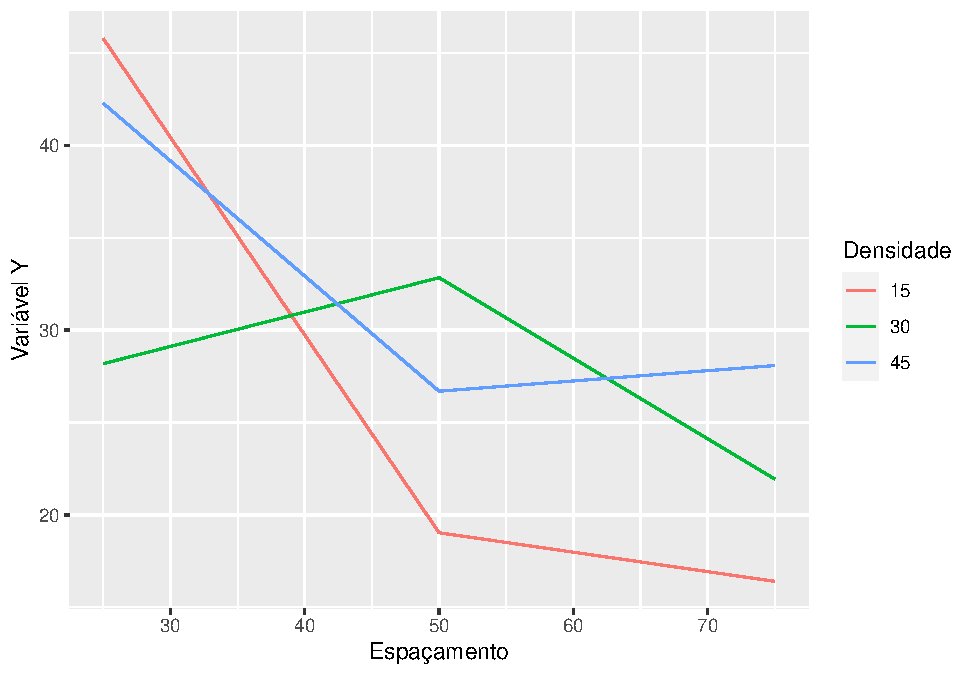
\includegraphics{curso_GIEU_files/figure-latex/unnamed-chunk-10-1.pdf}

\begin{Shaded}
\begin{Highlighting}[]
\NormalTok{dados }\OperatorTok\StringTok{ }
\StringTok{  }\KeywordTok{group_by}\NormalTok{(Espaçamento,Densidade) }\OperatorTok\StringTok{ }
\StringTok{  }\KeywordTok{summarise}\NormalTok{(}\DataTypeTok{Y =} \KeywordTok{mean}\NormalTok{(y)) }\OperatorTok\StringTok{ }
\StringTok{  }\KeywordTok{ggplot}\NormalTok{(}\KeywordTok{aes}\NormalTok{(}\DataTypeTok{x=}\NormalTok{Densidade, }\DataTypeTok{y=}\NormalTok{Y,}\DataTypeTok{col=}\KeywordTok{as.factor}\NormalTok{(Espaçamento)))}\OperatorTok{+}
\StringTok{  }\KeywordTok{geom_line}\NormalTok{()}\OperatorTok{+}
\StringTok{  }\KeywordTok{labs}\NormalTok{(}\DataTypeTok{x=}\StringTok{"Densidade"}\NormalTok{,}\DataTypeTok{y=}\StringTok{"Variável Y"}\NormalTok{,}\DataTypeTok{col=}\StringTok{"Espaçamento"}\NormalTok{)}
\end{Highlighting}
\end{Shaded}

\begin{verbatim}
## `summarise()` regrouping output by 'Espaçamento' (override with `.groups` argument)
\end{verbatim}

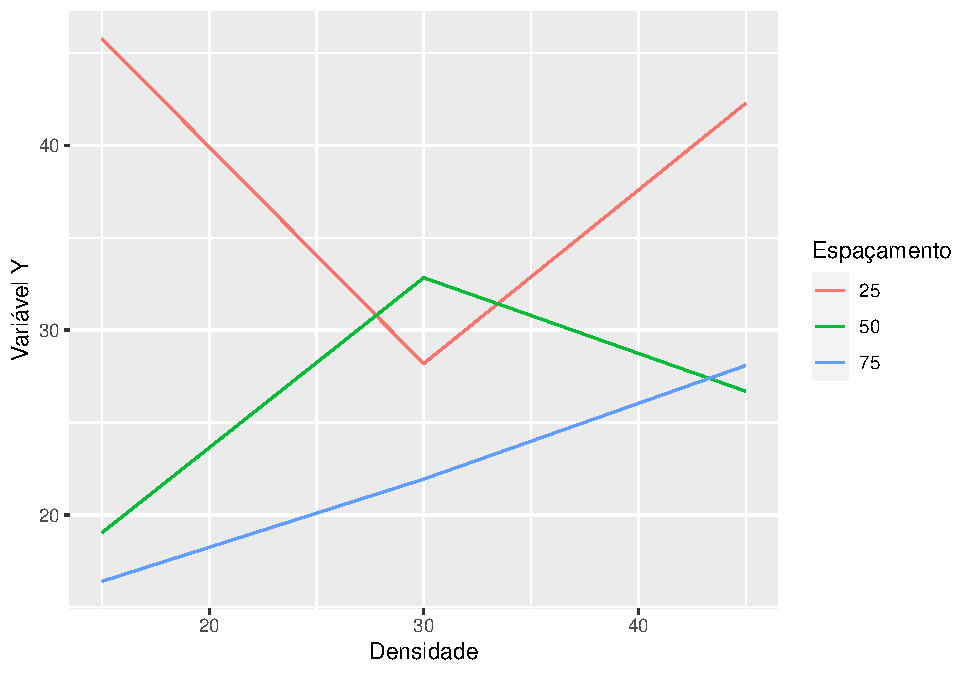
\includegraphics{curso_GIEU_files/figure-latex/unnamed-chunk-10-2.pdf}
\textbf{Analise considerando o delineamento de tratamentos}

\begin{Shaded}
\begin{Highlighting}[]
\NormalTok{mod <-}\StringTok{ }\KeywordTok{aov}\NormalTok{(y}\OperatorTok{~}\NormalTok{den }\OperatorTok{+}\StringTok{ }\NormalTok{esp }\OperatorTok{+}\StringTok{ }\NormalTok{den}\OperatorTok{:}\NormalTok{esp)}
\KeywordTok{anova}\NormalTok{(mod)}
\end{Highlighting}
\end{Shaded}

\begin{verbatim}
## Analysis of Variance Table
## 
## Response: y
##           Df  Sum Sq Mean Sq F value   Pr(>F)   
## den        2  150.53   75.26  1.1416 0.341378   
## esp        2 1347.49  673.75 10.2191 0.001083 **
## den:esp    4  860.09  215.02  3.2614 0.035405 * 
## Residuals 18 1186.75   65.93                    
## ---
## Signif. codes:  0 '***' 0.001 '**' 0.01 '*' 0.05 '.' 0.1 ' ' 1
\end{verbatim}

\textbf{Medias dos efeitos principais e da interação}

\begin{Shaded}
\begin{Highlighting}[]
\KeywordTok{model.tables}\NormalTok{(mod,}\DataTypeTok{type=}\StringTok{"means"}\NormalTok{)}
\end{Highlighting}
\end{Shaded}

\begin{verbatim}
## Tables of means
## Grand mean
##          
## 29.02222 
## 
##  den 
## den
##    15    30    45 
## 27.07 27.65 32.34 
## 
##  esp 
## esp
##    25    50    75 
## 38.74 26.19 22.14 
## 
##  den:esp 
##     esp
## den  25    50    75   
##   15 45.77 19.04 16.41
##   30 28.18 32.83 21.94
##   45 42.26 26.69 28.08
\end{verbatim}

\textbf{SE A INTERAÇÃO FOR SIGNIFICATIVA}

\textbf{Desdobramento de Doses dentro Inseticidas}

\begin{Shaded}
\begin{Highlighting}[]
\CommentTok{# Redefinindo o modelo para o estudo das interações}
\NormalTok{modab <-}\StringTok{ }\KeywordTok{aov}\NormalTok{(y}\OperatorTok{~}\NormalTok{esp}\OperatorTok{/}\NormalTok{den) }\CommentTok{# Colocar os Controles locais, blocos, se for o caso}
\KeywordTok{effects}\NormalTok{(modab)}
\end{Highlighting}
\end{Shaded}

\begin{verbatim}
##  (Intercept)        esp50        esp75  esp25:den30  esp50:den30  esp75:den30 
## -150.8038903  -10.4140056  -35.2000113   22.3858222  -14.0935810    0.4320422 
##  esp25:den45  esp50:den45  esp75:den45                                        
##    4.2927308    9.3733807  -14.2964469  -14.6589072   -4.4221698    8.5114134 
##                                                                               
##   -3.6891278    0.2827470   -6.8232618   -2.1185369   -0.8663283   -1.0888551 
##                                                                               
##   14.4060928   -7.7321698  -12.9235866   -4.1791278   -1.2172530   -7.0262618 
##                                        
##   13.6894631   -6.8953283    8.6941449 
## attr(,"assign")
## [1] 0 1 1 2 2 2 2 2 2
## attr(,"class")
## [1] "coef"
\end{verbatim}

\begin{Shaded}
\begin{Highlighting}[]
\KeywordTok{effects}\NormalTok{(modab)[}\DecValTok{4}\OperatorTok{:}\DecValTok{9}\NormalTok{]}
\end{Highlighting}
\end{Shaded}

\begin{verbatim}
## esp25:den30 esp50:den30 esp75:den30 esp25:den45 esp50:den45 esp75:den45 
##  22.3858222 -14.0935810   0.4320422   4.2927308   9.3733807 -14.2964469
\end{verbatim}

\begin{Shaded}
\begin{Highlighting}[]
\KeywordTok{summary}\NormalTok{(modab,}\DataTypeTok{split=}\KeywordTok{list}\NormalTok{(}\StringTok{"esp:den"}\NormalTok{=}\KeywordTok{list}\NormalTok{(}\DataTypeTok{Esp25=}\KeywordTok{c}\NormalTok{(}\DecValTok{1}\NormalTok{,}\DecValTok{4}\NormalTok{), }
                                         \DataTypeTok{Esp50=}\KeywordTok{c}\NormalTok{(}\DecValTok{2}\NormalTok{,}\DecValTok{5}\NormalTok{),}
                                         \DataTypeTok{Esp75=}\KeywordTok{c}\NormalTok{(}\DecValTok{3}\NormalTok{,}\DecValTok{6}\NormalTok{)}
\NormalTok{                                         ))) }
\end{Highlighting}
\end{Shaded}

\begin{verbatim}
##                  Df Sum Sq Mean Sq F value  Pr(>F)   
## esp               2 1347.5   673.7  10.219 0.00108 **
## esp:den           6 1010.6   168.4   2.555 0.05730 . 
##   esp:den: Esp25  2  519.6   259.8   3.940 0.03808 * 
##   esp:den: Esp50  2  286.5   143.2   2.173 0.14281   
##   esp:den: Esp75  2  204.6   102.3   1.551 0.23899   
## Residuals        18 1186.7    65.9                   
## ---
## Signif. codes:  0 '***' 0.001 '**' 0.01 '*' 0.05 '.' 0.1 ' ' 1
\end{verbatim}

\textbf{Desdobramento de Inseticida dentro de Dose}

\begin{Shaded}
\begin{Highlighting}[]
\CommentTok{# Redefinindo o modelo para o estudo das interações}
\NormalTok{modba <-}\StringTok{ }\KeywordTok{aov}\NormalTok{(y}\OperatorTok{~}\NormalTok{den}\OperatorTok{/}\NormalTok{esp) }\CommentTok{# Colocar os Controles locais, blocos, se for o caso}
\KeywordTok{effects}\NormalTok{(modba)}
\end{Highlighting}
\end{Shaded}

\begin{verbatim}
##  (Intercept)        den30        den45  den15:esp50  den30:esp50  den45:esp50 
## -150.8038903    5.0369674  -11.1873721   17.0372665  -10.9891465   11.9894669 
##  den15:esp75  den30:esp75  den45:esp75                                        
##   35.9548352    7.6477152   17.3656575  -13.4015598   -0.8481823    7.8234798 
##                                                                               
##   -5.2203439    0.1202090   -9.6712262   -3.3867486    0.9615199   -3.4279641 
##                                                                               
##   15.6634402   -4.1581823  -13.6115202   -5.7103439   -1.3797910   -9.8742262 
##                                        
##   12.4212514   -5.0674801    6.3550359 
## attr(,"assign")
## [1] 0 1 1 2 2 2 2 2 2
## attr(,"class")
## [1] "coef"
\end{verbatim}

\begin{Shaded}
\begin{Highlighting}[]
\KeywordTok{effects}\NormalTok{(modba)[}\DecValTok{4}\OperatorTok{:}\DecValTok{9}\NormalTok{]}
\end{Highlighting}
\end{Shaded}

\begin{verbatim}
## den15:esp50 den30:esp50 den45:esp50 den15:esp75 den30:esp75 den45:esp75 
##   17.037266  -10.989146   11.989467   35.954835    7.647715   17.365658
\end{verbatim}

\begin{Shaded}
\begin{Highlighting}[]
\KeywordTok{summary}\NormalTok{(modba,}\DataTypeTok{split=}\KeywordTok{list}\NormalTok{(}\StringTok{"den:esp"}\NormalTok{=}\KeywordTok{list}\NormalTok{(}\DataTypeTok{Den15=}\KeywordTok{c}\NormalTok{(}\DecValTok{1}\NormalTok{,}\DecValTok{4}\NormalTok{),}
                                        \DataTypeTok{Den30=}\KeywordTok{c}\NormalTok{(}\DecValTok{2}\NormalTok{,}\DecValTok{5}\NormalTok{),}
                                        \DataTypeTok{Den45=}\KeywordTok{c}\NormalTok{(}\DecValTok{3}\NormalTok{,}\DecValTok{6}\NormalTok{)}
\NormalTok{                                                ))) }
\end{Highlighting}
\end{Shaded}

\begin{verbatim}
##                  Df Sum Sq Mean Sq F value   Pr(>F)    
## den               2  150.5    75.3   1.142 0.341378    
## den:esp           6 2207.6   367.9   5.581 0.002021 ** 
##   den:esp: Den15  2 1583.0   791.5  12.005 0.000487 ***
##   den:esp: Den30  2  179.2    89.6   1.359 0.281954    
##   den:esp: Den45  2  445.3   222.7   3.377 0.056832 .  
## Residuals        18 1186.7    65.9                     
## ---
## Signif. codes:  0 '***' 0.001 '**' 0.01 '*' 0.05 '.' 0.1 ' ' 1
\end{verbatim}

\textbf{Utilizando o pacote ExpDes.pt, mais prático}

\begin{Shaded}
\begin{Highlighting}[]
\CommentTok{# Carregando o pacote par análise de variância}
\KeywordTok{library}\NormalTok{(ExpDes.pt)}
\NormalTok{caminho<-}\StringTok{"https://raw.githubusercontent.com/arpanosso/curso_GIEU/master/dados/crotalaria.txt"}
\NormalTok{d<-}\KeywordTok{read.table}\NormalTok{(caminho,}\DataTypeTok{h=}\OtherTok{TRUE}\NormalTok{)}
\NormalTok{esp<-}\KeywordTok{factor}\NormalTok{(d}\OperatorTok{$}\NormalTok{Espaçamento)}
\NormalTok{den<-}\KeywordTok{factor}\NormalTok{(d}\OperatorTok{$}\NormalTok{Densidade)}
\NormalTok{bloco<-}\KeywordTok{factor}\NormalTok{(d}\OperatorTok{$}\NormalTok{Bloco)}
\NormalTok{y<-d}\OperatorTok{$}\NormalTok{y}
\KeywordTok{fat2.dbc}\NormalTok{(esp,den,bloco,y,}\DataTypeTok{fac.names =} \KeywordTok{c}\NormalTok{(}\StringTok{"Espaçamento"}\NormalTok{, }\StringTok{"Densidade"}\NormalTok{))}
\end{Highlighting}
\end{Shaded}

\begin{verbatim}
## ------------------------------------------------------------------------
## Legenda:
## FATOR 1:  Espaçamento 
## FATOR 2:  Densidade 
## ------------------------------------------------------------------------
## 
## 
## Quadro da analise de variancia
## ------------------------------------------------------------------------
##                       GL     SQ QM      Fc   Pr>Fc
## Bloco                  2  114.4  3  0.8535 0.44444
## Espaçamento            2 1347.5  5 10.0527 0.00149
## Densidade              2  150.5  6  1.1230 0.34964
## Espaçamento*Densidade  4  860.1  2  3.2083 0.04101
## Residuo               16 1072.3  4                
## Total                 26 3544.9  1                
## ------------------------------------------------------------------------
## CV = 28.21 %
## 
## ------------------------------------------------------------------------
## Teste de normalidade dos residuos (Shapiro-Wilk)
## valor-p:  0.541538 
## De acordo com o teste de Shapiro-Wilk a 5% de significancia, os residuos podem ser considerados normais.
## ------------------------------------------------------------------------
## 
## 
## 
## Interacao significativa: desdobrando a interacao
## ------------------------------------------------------------------------
## 
## Desdobrando  Espaçamento  dentro de cada nivel de  Densidade 
## ------------------------------------------------------------------------
## ------------------------------------------------------------------------
## Quadro da analise de variancia
## ------------------------------------------------------------------------
##                          GL        SQ        QM      Fc  Pr.Fc
## Bloco                     2  114.4004  57.20020  0.8535 0.4444
## Densidade                 2  150.5283  75.26417   1.123 0.3496
## Espaçamento:Densidade 15  2 1583.0186 791.50931 11.8098  7e-04
## Espaçamento:Densidade 30  2  179.2489  89.62444  1.3372 0.2904
## Espaçamento:Densidade 45  2  445.3134 222.65669  3.3222 0.0621
## Residuo                  16 1072.3451  67.02157               
## Total                    26 3544.8547 136.34057               
## ------------------------------------------------------------------------
## 
## 
## 
##  Espaçamento  dentro do nivel  15  de  Densidade 
## ------------------------------------------------------------------------
## Teste de Tukey
## ------------------------------------------------------------------------
## Grupos Tratamentos Medias
## a     1   45.765 
##  b    2   19.03933 
##  b    3   16.408 
## ------------------------------------------------------------------------
## 
## 
##  Espaçamento  dentro do nivel  30  de  Densidade 
## 
## De acordo com o teste F, as medias desse fator sao estatisticamente iguais.
## ------------------------------------------------------------------------
##     Niveis     Medias
## 1        1   28.18333
## 2        2   32.83167
## 3        3   21.93900
## ------------------------------------------------------------------------
## 
## 
##  Espaçamento  dentro do nivel  45  de  Densidade 
## 
## De acordo com o teste F, as medias desse fator sao estatisticamente iguais.
## ------------------------------------------------------------------------
##     Niveis     Medias
## 1        1   42.26000
## 2        2   26.69267
## 3        3   28.08100
## ------------------------------------------------------------------------
## 
## 
## 
## Desdobrando  Densidade  dentro de cada nivel de  Espaçamento 
## ------------------------------------------------------------------------
## ------------------------------------------------------------------------
## Quadro da analise de variancia
## ------------------------------------------------------------------------
##                          GL        SQ        QM      Fc  Pr.Fc
## Bloco                     2  114.4004  57.20020  0.8535 0.4444
## Espaçamento               2 1347.4923 673.74615 10.0527 0.0015
## Densidade:Espaçamento 25  2  519.5526 259.77629   3.876 0.0424
## Densidade:Espaçamento 50  2  286.4893 143.24465  2.1373 0.1504
## Densidade:Espaçamento 75  2  204.5751 102.28753  1.5262 0.2474
## Residuo                  16 1072.3451  67.02157               
## Total                    26 3544.8547 136.34057               
## ------------------------------------------------------------------------
## 
## 
## 
##  Densidade  dentro do nivel  25  de  Espaçamento 
## ------------------------------------------------------------------------
## Teste de Tukey
## ------------------------------------------------------------------------
## Grupos Tratamentos Medias
## a     1   45.765 
## ab    3   42.26 
##  b    2   28.18333 
## ------------------------------------------------------------------------
## 
## 
##  Densidade  dentro do nivel  50  de  Espaçamento 
## 
## De acordo com o teste F, as medias desse fator sao estatisticamente iguais.
## ------------------------------------------------------------------------
##     Niveis     Medias
## 1        1   19.03933
## 2        2   32.83167
## 3        3   26.69267
## ------------------------------------------------------------------------
## 
## 
##  Densidade  dentro do nivel  75  de  Espaçamento 
## 
## De acordo com o teste F, as medias desse fator sao estatisticamente iguais.
## ------------------------------------------------------------------------
##     Niveis     Medias
## 1        1     16.408
## 2        2     21.939
## 3        3     28.081
## ------------------------------------------------------------------------
\end{verbatim}

\hypertarget{experimentos-em-parcelas-subdivididas}{%
\chapter{Experimentos em Parcelas Subdivididas}\label{experimentos-em-parcelas-subdivididas}}

\textbf{Introdução}

Os experimento em parcelas subdivididas, também conhecidos como ``Split-plot'', são utilizados quado, num mesmo ensaio, queremos testar os efeitos de 2 ou mais fatores, mas em condições experimentais um pouco diferentes daquelas utilizadas nos experimentos fatoriais.

Por exemplo:

\begin{itemize}
\tightlist
\item
  4 Variedades e 3 Níveis de Adubação\\
\item
  3 Níveis de Irrigação e 4 Níveis de Adubação\\
\item
  3 Espaçamentos e 4 densidades de Semeadura\\
  etc.
\end{itemize}

As unidade experimentais ou parcelas, são divididas em partes menores e iguais, chamadas de subparcelas.

As parcelas podem ser ditribuídas de acordo com um delineamento qualquer, ou seja, inteiramente ao acaso ou blocos casualizados. A principal característica deste delineamento é a casualiização dos tratamentos, que é feita em 2 estágios.

\begin{itemize}
\tightlist
\item
  No primeiro estágio, é feita a casualização dos níveis do fator testado, nas parcelas, de acordo com o delineamento adotado.
\item
  No segundo estágio, em cada parcela, é eita a casualização dos níveis do fator que será testados na subparcelas.
\end{itemize}

Denominamos de tratamentos principais ou tratamento primários, àqueles que são colocados nas parcelas, e de tratamento secundários ou subtratamentos àqueles que são colocados nas subparcelas.

Nesses experimento, temos 2 resíduos: O \textbf{resíduo a}, que serve como base de comparação para os tratamentos principais. e o \textbf{resíduo b}, que serve como base de comparação para os tratamentos secundários e para a interação \(P \times S\).

Em consequência do tipo de casualização feia, o erro experimentao devido aos tratamentos secundários (QM Resíduo b), geralmente é menor que o erro experimental devido aos tratamentos principais (QM Resíduo a).

Dessa maneira, os efeitos dos tratamentos principais são determinados com menor precisão que os efeitods dos tratamentos secundários.

Assim, por exemplo, num experimento em parcelas subdivididas, com os fatores: Adubação (tratamento principal-I) e Variedades (tratamento secundário-K), sendo utilzizados 2 níveis de Adubação (\(A_0\; e\; A_1\)) e 3 Variedades (\(V_1\;V_2\;e\; V_3\)), o esquema de casualização os tratamento , se o experimento fosse montado de acordo com o DBC, com 5 blocos (J), seria o seguinte.

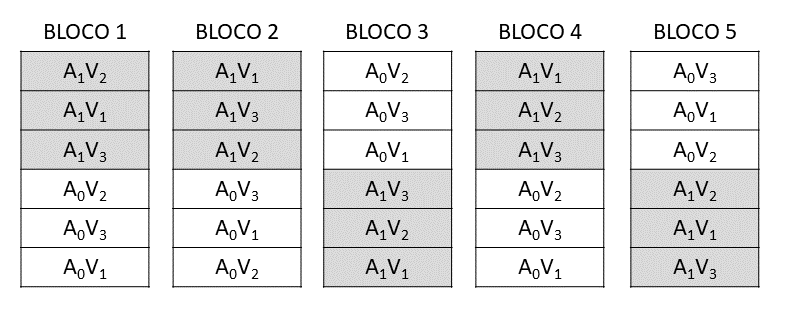
\includegraphics{psub1.png}
\textbf{Observação}: Caso este mesmo ensaio fosse montado de acordo com o esquema fatorial \(2 \times 3\) em 5 blocos, a casualização seria feita de modo diferente e, como exemplo, apresentamos o sorteio do delineamento seguinte:

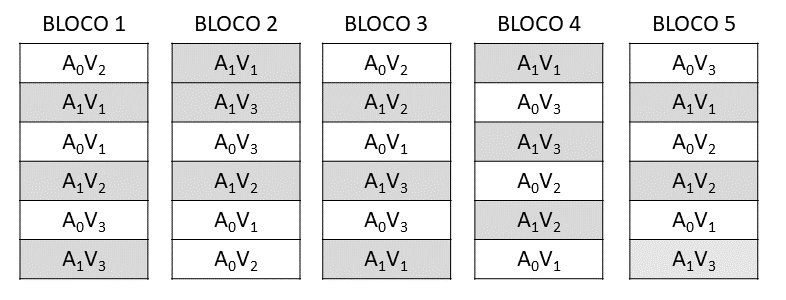
\includegraphics{fat1.png}

\textbf{Exemplo de Aplicação}

Para a obtenção da análise de variância de um experimento em parcelas subdivididas, vamos utilizar os dados obtidos do trabalho intitulado ``Efeito de épocas de plantio, sobre várias características agronômicas na cultura da soja (\emph{Glycine max}. (L.) Merril), variedades Santa Rosa e Viçoja, e Jaboticabal, SP'', realizado por K. YUYAMA (1976). Foram utilizadas 8 épocas de plantio (20/10/74, 30/10/74, 10/11/74, 20/11/74, 30/11/74, 10/12/47, 20/12/74 e 30/12/74) e duas variedade de soja (\(V_1\) = Viçoja e \(V_2\) = Santa Rosa). O ensaio foi montado de acordo com o delineamento em parcelas subdivididas, com as épocas de plantio nas parcelas, e as variedades nas subparcelas. Os resultados obtidos para produção de grãos (\(t\;ha^{-1}\)), foram os seguintes:

\begin{longtable}[]{@{}lcccc@{}}
\toprule
Tratamentos & Bloco 1 & Bloco 2 & Bloco 3 & Total\tabularnewline
\midrule
\endhead
\(E_1V_1\) & 2,9166 & 2,8833 & 2,4750 & 8,2749\tabularnewline
\(E_1V_2\) & 2,6416 & 3,6666 & 3,6166 & 9,9248\tabularnewline
\(E_2V_1\) & 3,4889 & 3,5833 & 3,3333 & 10,4055\tabularnewline
\(E_2V_2\) & 4,0583 & 4,3000 & 2,9083 & 11,2666\tabularnewline
\(E_3V_1\) & 2,3166 & 2,8666 & 2,4916 & 7,6748\tabularnewline
\(E_3V_2\) & 3,4500 & 3,7666 & 3,5333 & 10,7499\tabularnewline
\(E_4V_1\) & 2,7916 & 2,7583 & 3,1916 & 8,7415\tabularnewline
\(E_4V_2\) & 3,4166 & 2,7416 & 3,5083 & 9,6665\tabularnewline
\(E_5V_1\) & 3,5583 & 3,1583 & 2,7916 & 9,5082\tabularnewline
\(E_5V_2\) & 3,5000 & 3,1166 & 3,0916 & 9,7082\tabularnewline
\(E_6V_1\) & 2,7833 & 2,5166 & 2,1250 & 7,4249\tabularnewline
\(E_6V_2\) & 2,5583 & 2,5666 & 2,0416 & 7,1665\tabularnewline
\(E_7V_1\) & 2,3000 & 2,2083 & 2,0666 & 6,5749\tabularnewline
\(E_7V_2\) & 1,4250 & 1,9166 & 1,8750 & 5,2166\tabularnewline
\(E_8V_1\) & 1,1666 & 1,6916 & 1,4666 & 4,3248\tabularnewline
\(E_8V_2\) & 2,0083 & 1,7833 & 1,7416 & 5,5332\tabularnewline
Total & 44,3800 & 45,5242 & 42,2576 & \textbf{132,1618}\tabularnewline
\bottomrule
\end{longtable}

os dados estão disponíveis online em: \href{https://raw.githubusercontent.com/arpanosso/curso_GIEU/master/dados/sojapsub.txt}{sojapsub.txt}.

\textbf{Aplicação em R - Parcelas Sudivididas}


\includegraphics{R.png}

\begin{Shaded}
\begin{Highlighting}[]
\KeywordTok{require}\NormalTok{(ExpDes.pt)}
\NormalTok{caminho<-}\StringTok{"https://raw.githubusercontent.com/arpanosso/curso_GIEU/master/dados/sojapsub.txt"}
\NormalTok{d<-}\KeywordTok{read.table}\NormalTok{(caminho,}\DataTypeTok{h=}\NormalTok{T)}
\KeywordTok{psub2.dbc}\NormalTok{(d}\OperatorTok{$}\NormalTok{E,d}\OperatorTok{$}\NormalTok{V,d}\OperatorTok{$}\NormalTok{Bloco,d}\OperatorTok{$}\NormalTok{Y,}\DataTypeTok{fac.names =} \KeywordTok{c}\NormalTok{(}\StringTok{"Épocas"}\NormalTok{,}\StringTok{"Variedades"}\NormalTok{))}
\end{Highlighting}
\end{Shaded}

\begin{verbatim}
## ------------------------------------------------------------------------
## Legenda:
## FATOR 1 (parcela):  Épocas 
## FATOR 2 (subparcela):  Variedades 
## ------------------------------------------------------------------------
## 
## ------------------------------------------------------------------------
## $`Quadro da analise de variancia\n------------------------------------------------------------------------\n`
##                   GL      SQ QM      Fc  Pr(>Fc)    
## Épocas             7 19.0482  7 18.8291    4e-06 ***
## Bloco              2  0.3434  4  1.1882 0.333718    
## Erro a            14  2.0233  3                     
## Variedades         1  0.8276  6  9.4997 0.007142 ** 
## Épocas*Variedades  7  2.0370  5  3.3402 0.021671 *  
## Erro b            16  1.3939  2                     
## Total             47 25.6734  1                     
## ---
## Signif. codes:  0 '***' 0.001 '**' 0.01 '*' 0.05 '.' 0.1 ' ' 1
## 
## ------------------------------------------------------------------------
## CV 1 = 13.80697 %
## CV 2 = 10.71998 %
## 
## 
## 
## Interacao significativa: desdobrando a interacao
## ------------------------------------------------------------------------
## 
## Desdobrando  Épocas  dentro de cada nivel de  Variedades 
## ------------------------------------------------------------------------
##                              GL        SQ       QM        Fc valor.p
## Épocas : Variedades 1   7.00000  8.172581 1.167512 10.080441   4e-06
## Épocas : Variedades 2   7.00000 12.912557 1.844651 15.926946       0
## Erro combinado         27.28941  3.160659 0.115820                  
## ------------------------------------------------------------------------
## 
## 
##  Épocas dentro de Variedades 1
## ------------------------------------------------------------------------
## Teste de Tukey
## ------------------------------------------------------------------------
## Grupos Tratamentos Medias
## a     2   3.4685 
## ab    5   3.1694 
## abc   4   2.913833 
## abc   1   2.7583 
## abc   3   2.558267 
##  bc   6   2.474967 
##   cd      7   2.191633 
##    d      8   1.4416 
## ------------------------------------------------------------------------
## 
##  Épocas dentro de Variedades 2
## ------------------------------------------------------------------------
## Teste de Tukey
## ------------------------------------------------------------------------
## Grupos Tratamentos Medias
## a     2   3.755533 
## a     3   3.5833 
## a     1   3.308267 
## ab    5   3.236067 
## ab    4   3.222167 
##  bc   6   2.388833 
##   c   8   1.8444 
##   c   7   1.738867 
## ------------------------------------------------------------------------
## 
## 
## Desdobrando  Variedades  dentro de cada nivel de  Épocas 
## ------------------------------------------------------------------------
##                        GL       SQ       QM       Fc  valor.p
## Variedades : Épocas 1   1 0.453695 0.453695 5.207702 0.036511
## Variedades : Épocas 2   1 0.123582 0.123582 1.418528 0.251016
## Variedades : Épocas 3   1 1.576040 1.576040 18.09045 0.000607
## Variedades : Épocas 4   1 0.142604 0.142604 1.636871 0.218998
## Variedades : Épocas 5   1 0.006667 0.006667 0.076523 0.785608
## Variedades : Épocas 6   1 0.011128 0.011128 0.127737 0.725461
## Variedades : Épocas 7   1 0.307496 0.307496 3.529574 0.078628
## Variedades : Épocas 8   1 0.243372 0.243372 2.793523 0.114086
## Erro b                 16 1.393919 0.087120                  
## ------------------------------------------------------------------------
## 
## 
##  Variedades dentro de Épocas 1
## ------------------------------------------------------------------------
## Teste de Tukey
## ------------------------------------------------------------------------
## Grupos Tratamentos Medias
## a     2   3.308267 
##  b    1   2.7583 
## ------------------------------------------------------------------------
## ------------------------------------------------------------------------
## 
## 
##  Variedades dentro de Épocas 2
## ------------------------------------------------------------------------
## De acordo com o teste F, as medias desse fator sao estatisticamente iguais.
## ------------------------------------------------------------------------
##   Niveis   Medias
## 1      1 3.468500
## 2      2 3.755533
## ------------------------------------------------------------------------
## 
##  Variedades dentro de Épocas 3
## ------------------------------------------------------------------------
## Teste de Tukey
## ------------------------------------------------------------------------
## Grupos Tratamentos Medias
## a     2   3.5833 
##  b    1   2.558267 
## ------------------------------------------------------------------------
## ------------------------------------------------------------------------
## 
## 
##  Variedades dentro de Épocas 4
## ------------------------------------------------------------------------
## De acordo com o teste F, as medias desse fator sao estatisticamente iguais.
## ------------------------------------------------------------------------
##   Niveis   Medias
## 1      1 2.913833
## 2      2 3.222167
## ------------------------------------------------------------------------
## 
##  Variedades dentro de Épocas 5
## ------------------------------------------------------------------------
## De acordo com o teste F, as medias desse fator sao estatisticamente iguais.
## ------------------------------------------------------------------------
##   Niveis   Medias
## 1      1 3.169400
## 2      2 3.236067
## ------------------------------------------------------------------------
## 
##  Variedades dentro de Épocas 6
## ------------------------------------------------------------------------
## De acordo com o teste F, as medias desse fator sao estatisticamente iguais.
## ------------------------------------------------------------------------
##   Niveis   Medias
## 1      1 2.474967
## 2      2 2.388833
## ------------------------------------------------------------------------
## 
##  Variedades dentro de Épocas 7
## ------------------------------------------------------------------------
## De acordo com o teste F, as medias desse fator sao estatisticamente iguais.
## ------------------------------------------------------------------------
##   Niveis   Medias
## 1      1 2.191633
## 2      2 1.738867
## ------------------------------------------------------------------------
## 
##  Variedades dentro de Épocas 8
## ------------------------------------------------------------------------
## De acordo com o teste F, as medias desse fator sao estatisticamente iguais.
## ------------------------------------------------------------------------
##   Niveis Medias
## 1      1 1.4416
## 2      2 1.8444
## ------------------------------------------------------------------------
\end{verbatim}

\hypertarget{anuxe1lise-de-regressuxe3o}{%
\chapter{Análise de Regressão}\label{anuxe1lise-de-regressuxe3o}}

\textbf{Introdução}

Nos experimentos em que os tratamentos são quantitativos, como por exemplo, níveis crescentes de um adubo, doses crescentes de um inseticida, etc, muitas vezes existe uma correspondência funcional, denominada equação de regressão, que relaciona os valores dos tratamentos (X) com os dados analisados (Y).

Por exemplo, essa dependência pode ser notada no caso seguinte,onde X representa as doses de um adubo (\(kg\;h^{-1}\)) e y a produção de milho (\(kg\;h^{-1}\)).

\begin{longtable}[]{@{}cccccc@{}}
\toprule
X & 0 & 25 & 50 & 75 & 100\tabularnewline
\midrule
\endhead
Y & 2100 & 2600 & 3000 & 3550 & 4150\tabularnewline
\bottomrule
\end{longtable}

Verificamos, portanto ,que há uma tendência de aumento na produção à medida que aumentamos a quantidade de adubo aplicada.

Vejamos então, como fazer a análise de variância para o estudo da regressão. O método utilizado é denominado de método dos polinômios ortogonais, e é de fácil aplicação quanto os níveis de X são equidistantes, poixs permitem a utilização de coeficientes obtidos em tabelas.

\textbf{Obtenção da análise de variância, estudando-se os efeitos da regressão}

Para estudo da regressão, vamos utilizar os dados do trabalho: ``Efeito de doses de gesso na cultura do feijoeiro (\emph{Phaseolu vulgaris} L.)'', realizado por RAGAZZI (1979). Neste trabalho foram utilizadas 7 doses de gesso 0, 50, 100, 150, 200, 250, e 300 \(kg\;ha^{-1}\). Os resultados obtidos para peso de 1000 sementes, em gramas, são apresentados a seguir:

\begin{longtable}[]{@{}lccccc@{}}
\toprule
Tratamentos & Rep.~1 & Rep.~2 & Rep.~3 & Rep.~4 & Totais\tabularnewline
\midrule
\endhead
0 & 134,8 & 139,7 & 147,6 & 132,3 & 554,4\tabularnewline
50 & 161,7 & 157,7 & 150,3 & 144,7 & 614,4\tabularnewline
100 & 160,7 & 172,7 & 163,4 & 161,3 & 658,1\tabularnewline
150 & 169,8 & 168,2 & 160,7 & 161,0 & 659,7\tabularnewline
200 & 165,7 & 160,0 & 158,2 & 151,0 & 634,9\tabularnewline
250 & 171,8 & 157,3 & 150,4 & 160,4 & 639,9\tabularnewline
300 & 154,5 & 160,4 & 148,8 & 154,0 & 617,7\tabularnewline
\textbf{Totais} & & & & & \textbf{4379,1}\tabularnewline
\bottomrule
\end{longtable}

Os dados podem ser encontrados online em \href{https://raw.githubusercontent.com/arpanosso/curso_GIEU/master/dados/feijaoREG.txt}{feijaoREG.txt}

A análise de variância preliminar será realizada de acordo com o delineamento experimental utilizado. O Ensaio foi montado de acordo com o delineamento inteiramente casualizado, e portanto, a análise de variância preliminar, obtido de maneira usual,

Quadro de análise de variância preliminar:

\begin{longtable}[]{@{}lcccc@{}}
\toprule
Causas de Variação & GL & SQ & QM & F\tabularnewline
\midrule
\endhead
Tratamentos & 6 & 1941,83 & 323,64 & 7,67**\tabularnewline
Resíduo & 21 & 886,34 & 42,21 & --\tabularnewline
\textbf{Total} & \textbf{27} & \textbf{2828,17} & \textbf{--} & \textbf{--}\tabularnewline
\bottomrule
\end{longtable}

\textbf{Conclusão}: O teste F foi significativo ao nível de \(1\%\) de probabilidade, logo, rejeitamos a hipótese da nulidade (\(H_0\)), e concluímos que as doses de gesso aplicadas possuem efeitos diferentes sobre o peso de 1000 sementes.

No entanto, um caso como este, em que os tratamentos são quantitativos, e em mais de 2 níveis, uma análise mais detalhada deve levar em conta a regressão, desdobrando-se os 6 graus de liberdade de tratamentos em:

Regressão Linear\ldots\ldots..1 GL\\
Regressão Quadrática\ldots1 GL\\
Regressão Cúbica\ldots\ldots..1 GL\\
Regressão de 4º grau\ldots1 GL\\
Regressão de 5º grau\ldots1 GL\\
Regressão de 6º grau\ldots1 GL\\
---------------------------------------\\
(Tratamentos)\ldots\ldots\ldots\ldots(6) GL

Porém, as regressões de grau maior que 3º não tem interesse prático, de modo que, na análise de variância, podemos considerar as regress\textasciitilde es de graus maior que o 3º como uma única causa de variação, que denominamos de \textbf{Desvios da Regressão}. Assim, no nosso exemplo, temos:

\begin{longtable}[]{@{}lr@{}}
\toprule
Causas de Variação & GL\tabularnewline
\midrule
\endhead
Regressão Linear & 1\tabularnewline
Regressão Quadrática & 1\tabularnewline
Regressão Cúbica & 1\tabularnewline
Desvios da Regressão & 3\tabularnewline
(Tratamentos) & (6)\tabularnewline
Resíduo & 21\tabularnewline
Total & 27\tabularnewline
\bottomrule
\end{longtable}

Esta decomposição pode ser feita pelo métido dos polinômios ortogoais, e é de fácil aplicação quando as quantidades que determinam os tratamentos são igualmente espaçadas (equidistantes), o que ocorre no caso em estudo (0, 50, 100, 150, 20, 250, 300). Neste casos, os coeficientes dos polinômios ortogonais são obtidos em tabelas, como a seguintes:

\textbf{CONCLUSÃO}:\\
Os testes F para a regressão linear e regressão quadrática foram significativos ao nível de \(1\%\) de probabilidade, indicando que é possível estabelecer uma relação funcional entre a dose de gesso (\(X\)) e o peso de 1000 sementes do feijoeiro (\(Y\)).

A equação de regressão que melhor se ajusta aos dados é a correspondente à \textbf{REGRESSÃO DE MAIS ALTO GRAU} cujo teste F soi significativo.

Assim, sendo, no nosso exemplo, a equação que melhor se ajusta é a de 2º grau (Quadrática).

Quando o teste F para \textbf{Desvios da Regressão for significativo}, isto indica que \textbf{existe alguma regressão significativa de grau maior que o 3º} e, se tivermos interesse em estudá-la, devemos desdobrar os graus de liberdade de Desvio da Regressão.

\textbf{Gráfico da Regressão Ajustada}

Podemos fazer uma verificação do ajuste da equação de regressão, calculando os valores esperados de (\(\hat{Y}_i\)) por meio da equação de regressão ajustada, e os valores observados (\(\bar{Y}_{i\;Obs}\)) por meio das médias dos tratamentos.

Devemos verificar que \(\sum_{i=1}^I\bar{Y}_{i~Obs}=\sum_{i=1}^I\hat{Y}_{i}\). estes valores podem também ser utilizados para a construção do gráfico de regressão ajustada.

No nosso exemplo, temos:

\begin{longtable}[]{@{}lcc@{}}
\toprule
Dose de Gesso (X) & \(\bar{Y}_{i~Obs}\) & \(\hat{Y}_i\)\tabularnewline
\midrule
\endhead
0 & 138,60 & 140,78\tabularnewline
50 & 153,60 & 152,51\tabularnewline
100 & 164,53 & 160,32\tabularnewline
150 & 164,93 & 164,22\tabularnewline
200 & 158,73 & 164,20\tabularnewline
250 & 159,98 & 160,27\tabularnewline
300 & 154,43 & 152,42\tabularnewline
\textbf{Total} & \textbf{1094,80} & \textbf{1094,72}\tabularnewline
\bottomrule
\end{longtable}

\textbf{Aplicação em R - Análise de Regressão}


\includegraphics{R.png}

\begin{Shaded}
\begin{Highlighting}[]
\KeywordTok{require}\NormalTok{(ExpDes.pt)}
\NormalTok{caminho<-}\StringTok{"https://raw.githubusercontent.com/arpanosso/curso_GIEU/master/dados/feijaoREG.txt"}
\NormalTok{d<-}\KeywordTok{read.table}\NormalTok{(caminho,}\DataTypeTok{h=}\NormalTok{T)}
\CommentTok{# Análise de Variância}
\KeywordTok{dic}\NormalTok{(d}\OperatorTok{$}\NormalTok{trat,d}\OperatorTok{$}\NormalTok{y,}\DataTypeTok{quali =} \OtherTok{FALSE}\NormalTok{)}
\end{Highlighting}
\end{Shaded}

\begin{verbatim}
## ------------------------------------------------------------------------
## Quadro da analise de variancia
## ------------------------------------------------------------------------
##            GL      SQ QM    Fc      Pr>Fc
## Tratamento  6 1941.83  2 7.668 0.00018763
## Residuo    21  886.34  3                 
## Total      27 2828.17  1                 
## ------------------------------------------------------------------------
## CV = 4.15 %
## 
## ------------------------------------------------------------------------
## Teste de normalidade dos residuos 
## Valor-p:  0.5471519 
## De acordo com o teste de Shapiro-Wilk a 5% de significancia, os residuos podem ser considerados normais.
## ------------------------------------------------------------------------
## 
## ------------------------------------------------------------------------
## Teste de homogeneidade de variancia 
## valor-p:  0.3337639 
## De acordo com o teste de bartlett a 5% de significancia, as variancias podem ser consideradas homogeneas.
## ------------------------------------------------------------------------
## 
## Ajuste de modelos polinomiais de regressao
## ------------------------------------------------------------------------
## 
## Modelo Linear
## =========================================
##    Estimativa Erro.padrao   tc    valor.p
## -----------------------------------------
## b0  150.5652    2.2134    68.0255    0   
## b1   0.0389     0.0123    3.1664  0.0046 
## -----------------------------------------
## 
## R2 do modelo linear
## --------
## 0.217915
## --------
## 
## Analise de variancia do modelo linear
## =========================================================
##                      GL     SQ        QM     Fc   valor.p
## ---------------------------------------------------------
## Efeito linear        1   423.1544  423.1544 10.03 0.00465
## Desvios de Regressao 5  1,518.6780 303.7356  7.2  0.00046
## Residuos             21  886.3375  42.2066               
## ---------------------------------------------------------
## ------------------------------------------------------------------------
## 
## Modelo quadratico
## =========================================
##    Estimativa Erro.padrao   tc    valor.p
## -----------------------------------------
## b0  140.7839    2.8354    49.6527    0   
## b1   0.2736     0.0443    6.1812     0   
## b2  -0.0008     0.0001    -5.5196 0.00002
## -----------------------------------------
## 
## R2 do modelo quadratico
## --------
## 0.880095
## --------
## 
## Analise de variancia do modelo quadratico
## ===========================================================
##                      GL     SQ         QM      Fc   valor.p
## -----------------------------------------------------------
## Efeito linear        1   423.1544   423.1544  10.03 0.00465
## Efeito quadratico    1  1,285.8430 1,285.8430 30.47  2e-05 
## Desvios de Regressao 4   232.8346   58.2087   1.38  0.27505
## Residuos             21  886.3375   42.2066                
## -----------------------------------------------------------
## ------------------------------------------------------------------------
## 
## Modelo cubico
## =========================================
##    Estimativa Erro.padrao   tc    valor.p
## -----------------------------------------
## b0  138.2423    3.1302    44.1645    0   
## b1   0.4431     0.0989    4.4812  0.0002 
## b2  -0.0023     0.0008    -2.8551 0.0095 
## b3  0.000003       0      1.9166  0.0690 
## -----------------------------------------
## 
## R2 do modelo cubico
## --------
## 0.959938
## --------
## 
## Analise de variancia do modelo cubico
## ===========================================================
##                      GL     SQ         QM      Fc   valor.p
## -----------------------------------------------------------
## Efeito linear        1   423.1544   423.1544  10.03 0.00465
## Efeito quadratico    1  1,285.8430 1,285.8430 30.47  2e-05 
## Efeito cubico        1   155.0417   155.0417  3.67   0.069 
## Desvios de Regressao 3   77.7930    25.9310   0.61  0.61327
## Residuos             21  886.3375   42.2066                
## -----------------------------------------------------------
## ------------------------------------------------------------------------
\end{verbatim}

\begin{Shaded}
\begin{Highlighting}[]
\CommentTok{# Construção do gráfico}
\NormalTok{X<-}\KeywordTok{seq}\NormalTok{(}\DecValTok{0}\NormalTok{,}\DecValTok{300}\NormalTok{,}\DecValTok{50}\NormalTok{)}
\NormalTok{Y<-}\KeywordTok{tapply}\NormalTok{(d}\OperatorTok{$}\NormalTok{y, d}\OperatorTok{$}\NormalTok{trat, mean)}
\KeywordTok{plot}\NormalTok{(Y}\OperatorTok{~}\NormalTok{X,}
     \DataTypeTok{las=}\DecValTok{1}\NormalTok{,}
     \DataTypeTok{pch=}\DecValTok{21}\NormalTok{,}\DataTypeTok{col=}\StringTok{"black"}\NormalTok{,}\DataTypeTok{bg=}\StringTok{"gray"}\NormalTok{,}\DataTypeTok{cex=}\FloatTok{1.3}\NormalTok{,}
     \DataTypeTok{xlab=}\StringTok{"Dose de Gesso (kg/ha)"}\NormalTok{,}
     \DataTypeTok{ylab=}\StringTok{"Peso de 1000 sementes (g)"}
\NormalTok{);}\KeywordTok{curve}\NormalTok{(}\FloatTok{140.7836+0.2737}\OperatorTok{*}\NormalTok{x}\FloatTok{-0.000783}\OperatorTok{*}\NormalTok{x}\OperatorTok{^}\DecValTok{2}\NormalTok{,}\DataTypeTok{add=}\OtherTok{TRUE}\NormalTok{,}\DataTypeTok{col=}\StringTok{"red"}\NormalTok{,}\DataTypeTok{lwd=}\DecValTok{2}\NormalTok{)}
\KeywordTok{text}\NormalTok{(}\DecValTok{155}\NormalTok{,}\DecValTok{145}\NormalTok{,}\StringTok{"140.7836+0.2737X-0.000783X²\textbackslash{}nR²=0.8801"}\NormalTok{)}
\end{Highlighting}
\end{Shaded}

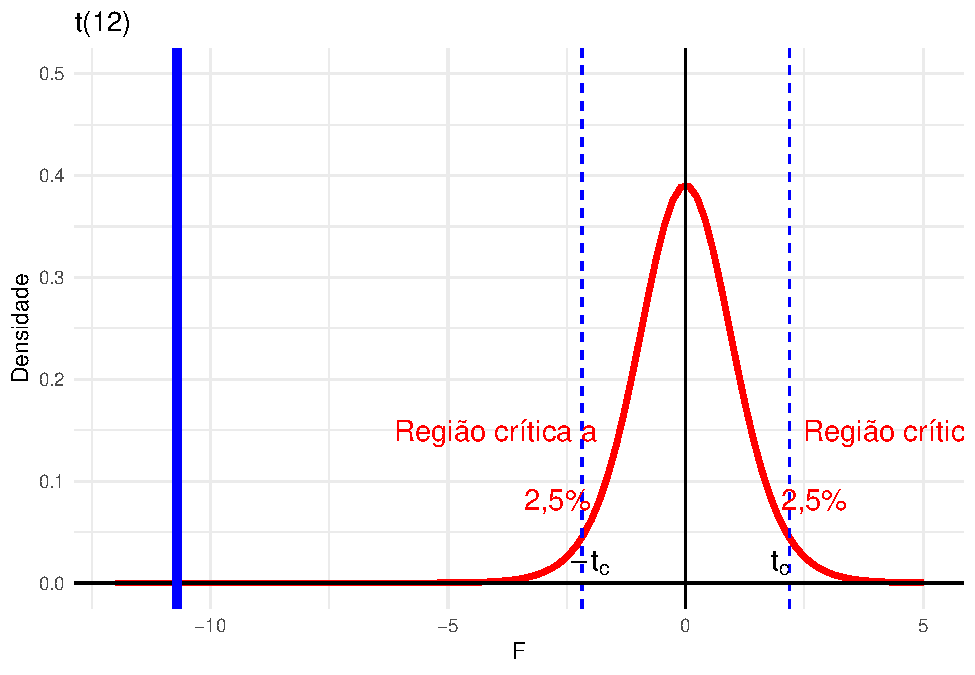
\includegraphics{curso_GIEU_files/figure-latex/unnamed-chunk-17-1.pdf}

Gráfico 1. relação entre o Peso de 1000 sementes e a dose de gesso aplicada.

  \bibliography{book.bib,packages.bib}

\end{document}
